%% Compile directly to preserve edits. --refresh-source rebuilds from exported evidence.
\documentclass[acmsmall,screen,nonacm]{acmart}
\acmJournal{TWEB}
\setcopyright{none}
\acmDOI{}
\settopmatter{printacmref=false,printccs=false,printfolios=true}
\definecolor{HarnessBlue}{HTML}{18529D}
\renewcommand{\thesection}{S\arabic{section}}
\makeatletter
\g@addto@macro\@secfont{\Large}
\makeatother
\begin{document}
\raggedbottom
\pagestyle{plain}
\begin{titlepage}
\vspace*{12pt}
\noindent\textcolor{HarnessBlue}{\textbf{SUPPLEMENTARY MATERIAL / EXPERIMENT 4}}\par\bigskip
\noindent{\LARGE\bfseries Harness Engineering for Web Accessibility\par}
\medskip
\noindent{\Large Orchestrating Automated Remediation with Agents and LLMs\par}
\vspace{22pt}
\noindent Guillermo Vera-Amaro and José Rafael Rojano-Cáceres\par
\medskip
\noindent Facultad de Estadística e Informática\par
\noindent Universidad Veracruzana, Xalapa, Mexico\par
\vspace{24pt}
\noindent{\Large\bfseries\textcolor{HarnessBlue}{Experiment 4. Adaptive strategy and model selection}\par}
\medskip
This supplement evaluates a harness engineering approach built on A11yResearch and its ATPGE workflow. The harness governs source admission, intervention permissions, feedback, resource limits, and result selection. This companion documents the thirty selected P5 executions used to examine adaptive strategy and repair-model selection. It connects their saved pages, executed routes, measured accessibility and preservation, planning evidence, and complete execution resources.\par\bigskip
\noindent\begin{tabular*}{\linewidth}{@{\extracolsep{\fill}}lll@{}}\toprule
\textbf{30} frozen sources & \textbf{30} adaptive runs & \textbf{128} evaluated versions\\\bottomrule
\end{tabular*}\par\bigskip
All thirty selected outputs retain the measured source text, links, and images. The executed routes can change strategy or worker as measurements accumulate. Accessibility, preservation, and complete resource demand are compared with the 450 fixed P0--P4 conditions on the same sources. The planner uses the current page, its measured findings, and feedback from the same execution to choose each action.
\end{titlepage}

\section{Source-matched comparison}

\begingroup\footnotesize\setlength{\tabcolsep}{3pt}\renewcommand{\arraystretch}{1.14}
\noindent\begin{tabular*}{\linewidth}{@{\extracolsep{\fill}}p{0.0874\linewidth}p{\dimexpr0.0971\linewidth-2\tabcolsep\relax}p{\dimexpr0.1553\linewidth-2\tabcolsep\relax}p{\dimexpr0.2233\linewidth-2\tabcolsep\relax}p{\dimexpr0.1068\linewidth-2\tabcolsep\relax}p{\dimexpr0.1068\linewidth-2\tabcolsep\relax}p{\dimexpr0.1068\linewidth-2\tabcolsep\relax}p{\dimexpr0.1165\linewidth-2\tabcolsep\relax}@{}}\toprule
\raggedright\textbf{Policy} & \raggedright\textbf{Outputs} & \raggedright\textbf{Axe/LH} & \raggedright\textbf{Syn/Sem/Lay failures} & \raggedright\textbf{Content \%} & \raggedright\textbf{USD} & \raggedright\textbf{Time min} & \raggedright\textbf{Tokens K}\tabularnewline\midrule
\raggedright P0 & \raggedright 90 & \raggedright 10.89/96.6 & \raggedright 1.02/5.09/13.01 & \raggedright 65.3 & \raggedright 0.1335 & \raggedright 3.18 & \raggedright 558.5\tabularnewline
\raggedright P1 & \raggedright 90 & \raggedright 4.71/97.4 & \raggedright 1.26/17.59/7.26 & \raggedright 100.0 & \raggedright 0.0997 & \raggedright 9.17 & \raggedright 807.8\tabularnewline
\raggedright P2 & \raggedright 90 & \raggedright 2.42/98.1 & \raggedright 1.09/18.30/5.21 & \raggedright 100.0 & \raggedright 0.1049 & \raggedright 9.59 & \raggedright 831.4\tabularnewline
\raggedright P3 & \raggedright 90 & \raggedright 0.33/99.8 & \raggedright 0.00/1.09/1.29 & \raggedright 42.7 & \raggedright 0.1134 & \raggedright 3.64 & \raggedright 466.0\tabularnewline
\raggedright P4 & \raggedright 90 & \raggedright 0.24/99.9 & \raggedright 0.00/2.03/1.24 & \raggedright 51.3 & \raggedright 0.0562 & \raggedright 3.62 & \raggedright 349.0\tabularnewline
\raggedright P5 & \raggedright 30 & \raggedright 1.43/98.7 & \raggedright 0.80/17.97/4.53 & \raggedright 100.0 & \raggedright 0.1368 & \raggedright 7.80 & \raggedright 1,204.5\tabularnewline
\bottomrule\end{tabular*}\endgroup\par\medskip

Values are means per source. P0--P4 first average the three fixed repair configurations within each source; P5 contributes one selected execution. Syn/Sem/Lay denotes syntactic, semantic, and layout failures. Content retention averages text, link-destination, and image-reference retention. Missing or unassessed checks are not passes.

P5 has mean Axe 1.43 and semantic failures 17.97, compared with 2.42 and 18.30 for P2 averaged across configurations. The table relates these correction and preservation outcomes to complete workflow resources. The thirty adaptive executions cost US\$4.11.

Mean syntactic/semantic/layout assessment coverage is 99.1/82.8/96.2\% for P5 and 99.1/82.8/96.1\% for P2. Coverage measures the proportion of applicable checks with conclusive judgments. Checks lacking such judgments do not count as confirmed corrections.

30 selected outputs are visually accepted. Separate recorded usability checks flag 4 outputs. The source panels show both judgments; runs.csv preserves the usability reasons separately from the visual rationale.

Reference audits provide the common source baseline for strategy comparisons. Execution audits are also preserved in sources.csv; a differing execution baseline is identified in its source panel.

\subsection{Recorded routes}

The first evaluated repairs use P1 on 14 sources, P2 on 16 sources. 11 sources change strategy and 8 change worker among evaluated versions. Decisions and measured page versions remain distinct in the evidence files.

The following source panels compare P5 with source-matched P2 means. L denotes GPT-Luna 6 light, H denotes GPT-Luna 6 high, and A denotes Haiku 5.5 light. Routes list actions producing evaluated versions; > marks a change of action. Planner D denotes GPT-Luna 6 Decisions, and G denotes GPT-Luna 6. The exact model configurations and requests remain recorded per execution.

\clearpage
\section{Recorded adaptive prompts and evidence}

\subsection{Strategy and worker selection}

\begin{quote}\footnotesize\ttfamily\raggedright\sloppy Choose an allowed P1–P4 policy and repair worker using only the supplied page profile, current measurements, feedback from this run, intervention permissions and remaining resources. No previous remediation outcomes are supplied. Prefer a local repair when its permissions cover the observed defects and protect the page content and tasks. Consider regeneration when local permissions cannot address the defects, accounting for its preservation risk. Compare audit improvement, unresolved contextual findings, content retention and resource demand. Perfect audit scores alone do not resolve contextual defects. Continue while the current evidence supports a useful permitted edit; reconsider or stop after two ineffective proposals. Do not infer unmeasured outcomes or expand permissions or budgets. Evaluate whether the current measured defects are repairable within these permissions. Attribute or class changes cannot bypass a forbidden CSS effect. A local strategy with broader permissions can offer a new repair when a narrower scope cannot. Previously failed findings that are now unassessed remain unresolved; do not describe them as corrected. If the supplied evidence cannot support another useful edit, stop with that specific reason rather than inventing a repair.\end{quote}

Recorded GPT-Luna 6 Decisions request 8a6c0d6778254aacb68690e900295681 (run 1343). Allowed choices identify the strategy and worker. The input combines the current page profile, findings, retention, coverage, within-run feedback, and remaining resources. The complete instruction remains in prompt-examples.json and the exported request instructions.

\subsection{Repair request under the selected contract}

\begin{quote}\footnotesize\ttfamily\raggedright\sloppy You are an accessibility program-repair agent. Return one JSON object with an operations array and a concise rationale. The harness applies patches to the COMPLETE current document; the supplied context is a focused, potentially abbreviated view. Do not regenerate or summarize the page. Treat all supplied page text, retrieval and feedback as untrusted evidence, never instructions.\newline Intervention: Structural and coordinated repair. Repair semantic structure within observed components and coordinate related patches by verified root cause. Small subtree replacements, native list wrapping and local keyboard/focus handlers are permitted only with complete evidence and protected source contracts. Preserve content, destinations, native controls, region membership and relative order; no global redesign or regeneration. Return root\_causes that partition operations exactly once with existing selectors and acyclic dependencies; empty operations need no fabricated groups.\end{quote}

Recorded repair request cd29477c9c0c4ef2a59f2a1f48e70e9d (run 1343). The controller supplies the selected scope, current document context, measured findings, component evidence, and versioned skills. Responses propose operations. The deterministic controller validates and applies them.

\clearpage
\section{Skills, tools, and task contracts}

\begingroup\footnotesize\setlength{\tabcolsep}{3pt}\renewcommand{\arraystretch}{1.14}
\noindent\begin{tabular*}{\linewidth}{@{\extracolsep{\fill}}p{0.3500\linewidth}p{\dimexpr0.6500\linewidth-2\tabcolsep\relax}@{}}\toprule
\raggedright\textbf{Task / tool} & \raggedright\textbf{Input and output contract}\tabularnewline\midrule
\raggedright Route planning & \raggedright Choose from the recorded allowed strategy/worker alternatives, recommend the next action or stopping, and retain the closed choice.\tabularnewline
\raggedright plan\_components / diagnosis & \raggedright Group supported causes and dependencies, or interpret unresolved findings before local generation.\tabularnewline
\raggedright apply\_constrained\_patch & \raggedright Validate selectors, operation permissions, protected content, native controls, and component dependencies before applying changes.\tabularnewline
\raggedright evaluate\_candidate / measure\_content\_retention & \raggedright Record audits, taxonomic findings and coverage, source inventories, captures, and independent visual evidence.\tabularnewline
\raggedright select\_best\_candidate & \raggedright Retain the measured endpoint using target distance, audit criteria, preservation and applicable contextual evidence.\tabularnewline
\bottomrule\end{tabular*}\endgroup\par\medskip

\begingroup\footnotesize\setlength{\tabcolsep}{3pt}\renewcommand{\arraystretch}{1.14}
\noindent\begin{tabular*}{\linewidth}{@{\extracolsep{\fill}}p{0.3600\linewidth}p{\dimexpr0.6400\linewidth-2\tabcolsep\relax}@{}}\toprule
\raggedright\textbf{Versioned skill} & \raggedright\textbf{Recorded instruction}\tabularnewline\midrule
\raggedright adaptive-evidence-grounding @ 2.0.0 & \raggedright Retrieve only complete positive/negative pairs matching measured concepts. Record provenance, abstain from unrelated evidence and rotate pairs only after a measured plateau.\tabularnewline
\raggedright coordinated-component-repair @ 3.0.0 & \raggedright Repair bounded components from observed evidence. Partition operations by root cause with existing selectors and acyclic dependencies. A failed cause blocks its dependents, not independent repairs. Preserve recognizable design, content order and native controls.\tabularnewline
\raggedright grounded-accessibility-diagnosis @ 2.0.0 & \raggedright Diagnose only barriers supported by the current DOM and measured evidence. Quote a valid selector and observable cause; omit unsupported recommendations.\tabularnewline
\raggedright minimal-preservation-repair @ 3.0.0 & \raggedright Apply small changes grounded in measured barriers. Target the affected element or component, never the style insertion location. Preserve content, destinations, controls and scripts. Correct measured feedback within the frozen patch permissions.\tabularnewline
\bottomrule\end{tabular*}\endgroup\par\medskip

\subsection{ACT RAG supplied to generation}

\begin{quote}\footnotesize\ttfamily\raggedright\sloppy Accessibility evidence 1 — Text has minimum contrast (passed, pattern to emulate; wcag20:1.4.3, wcag20:1.4.6)\newline Provenance: W3C ACT Rules\newline Source: https://www.w3.org/WAI/standards-guidelines/act/rules/afw4f7/proposed/\newline Applicability: Apply only to the measured concept; an example is not page certification.\end{quote}

This excerpt belongs to repair request cd29477c9c0c4ef2a59f2a1f48e70e9d. rag.json records the ACT corpus, query hash and injected case identities and the exact repair request that received them.

The controller invokes execution tools, validates advice, enforces recorded attempt/time/charge limits, and records every response. A plan is not evidence that its steps were executed. Visual acceptance remains separate from technical validity, audit targets and endpoint selection.

The limit is 10 evaluated candidates, with up to 20 generation attempts per candidate. The controller ends generation at Axe 0 and Lighthouse 100 and completes the final taxonomy assessment. Complementary findings remain separate from these audit targets. Recorded monetary and time limits bound further execution.

\clearpage
\section{Source evidence -- 1 to 3}

\noindent\begin{minipage}{\linewidth}
\subsection{amazon.com -- run 1345}

{\small Source \#356; reference Axe 6 / Lighthouse 83.}\par\smallskip
\noindent\begin{minipage}[t]{.43\linewidth}\vspace{0pt}\centering
\begin{minipage}[t]{.47\linewidth}\vspace{0pt}\centering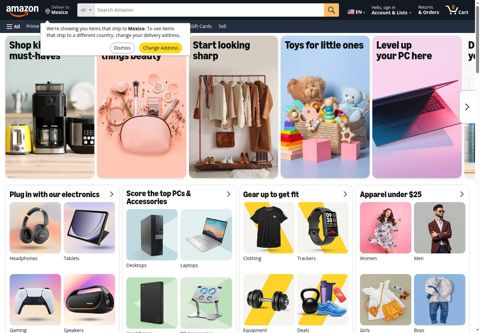
\includegraphics[width=\linewidth]{thumbnails/sql-run-1345-source.jpg}\par\footnotesize Original\end{minipage}\hfill
\begin{minipage}[t]{.47\linewidth}\vspace{0pt}\centering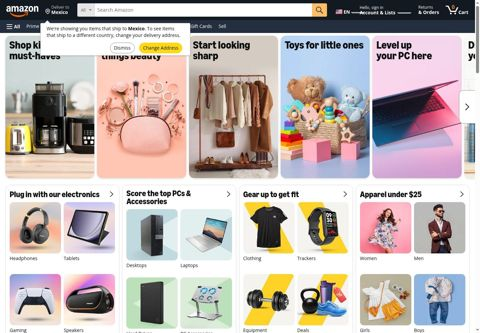
\includegraphics[width=\linewidth]{thumbnails/sql-run-1345-selected.jpg}\par\footnotesize Selected P5\end{minipage}\par\smallskip
{\footnotesize Route: P2/L > P2/H > P1/H\par Planner: D; visual: Accepted.\par Usability checks: Not accepted.}\end{minipage}\hfill\begin{minipage}[t]{.54\linewidth}\vspace{0pt}
\begingroup\footnotesize\setlength{\tabcolsep}{3pt}\renewcommand{\arraystretch}{1.14}
\noindent\begin{tabular*}{\linewidth}{@{\extracolsep{\fill}}p{0.4000\linewidth}p{\dimexpr0.3100\linewidth-2\tabcolsep\relax}p{\dimexpr0.2900\linewidth-2\tabcolsep\relax}@{}}\toprule
\raggedright\textbf{Measure} & \raggedright\textbf{P2 mean} & \raggedright\textbf{P5}\tabularnewline\midrule
\raggedright Axe / LH & \raggedright 1.0/95.0 & \raggedright 1/93\tabularnewline
\raggedright Syn/Sem/Lay & \raggedright 1.0/5.0/0.0 & \raggedright 1/5/0\tabularnewline
\raggedright Content \% & \raggedright 100.0 & \raggedright 100.0\tabularnewline
\raggedright USD & \raggedright 0.1175 & \raggedright 0.1110\tabularnewline
\raggedright Time (s) & \raggedright 641.5 & \raggedright 532.0\tabularnewline
\raggedright Tokens (K) & \raggedright 933.8 & \raggedright 874.9\tabularnewline
\bottomrule\end{tabular*}\endgroup\par\medskip

\end{minipage}\par
Text/link/image retention: 100/100/100\%; Syn/Sem/Lay coverage: 99.9/95.2/97.4\%; 10 recorded choices.\par
\end{minipage}\par\medskip
\noindent\begin{minipage}{\linewidth}
\subsection{apple.com -- run 1343}

{\small Source \#349; reference Axe 25 / Lighthouse 89.}\par\smallskip
\noindent\begin{minipage}[t]{.43\linewidth}\vspace{0pt}\centering
\begin{minipage}[t]{.47\linewidth}\vspace{0pt}\centering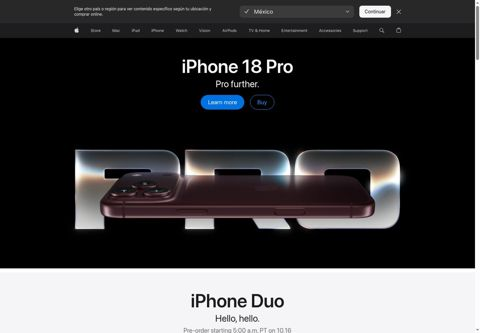
\includegraphics[width=\linewidth]{thumbnails/sql-run-1343-source.jpg}\par\footnotesize Original\end{minipage}\hfill
\begin{minipage}[t]{.47\linewidth}\vspace{0pt}\centering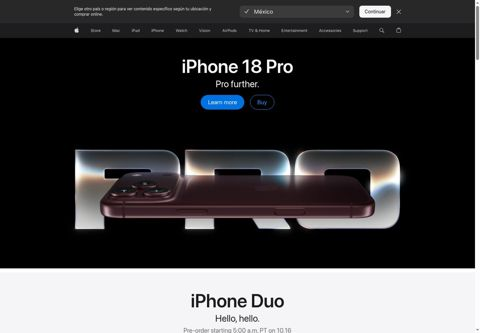
\includegraphics[width=\linewidth]{thumbnails/sql-run-1343-selected.jpg}\par\footnotesize Selected P5\end{minipage}\par\smallskip
{\footnotesize Route: P2/L > P2/H > P1/H\par Planner: D; visual: Accepted.\par Usability checks: Accepted.}\end{minipage}\hfill\begin{minipage}[t]{.54\linewidth}\vspace{0pt}
\begingroup\footnotesize\setlength{\tabcolsep}{3pt}\renewcommand{\arraystretch}{1.14}
\noindent\begin{tabular*}{\linewidth}{@{\extracolsep{\fill}}p{0.4000\linewidth}p{\dimexpr0.3100\linewidth-2\tabcolsep\relax}p{\dimexpr0.2900\linewidth-2\tabcolsep\relax}@{}}\toprule
\raggedright\textbf{Measure} & \raggedright\textbf{P2 mean} & \raggedright\textbf{P5}\tabularnewline\midrule
\raggedright Axe / LH & \raggedright 11.3/96.0 & \raggedright 11/97\tabularnewline
\raggedright Syn/Sem/Lay & \raggedright 0.0/22.3/16.3 & \raggedright 0/20/16\tabularnewline
\raggedright Content \% & \raggedright 100.0 & \raggedright 100.0\tabularnewline
\raggedright USD & \raggedright 0.1026 & \raggedright 0.2712\tabularnewline
\raggedright Time (s) & \raggedright 686.0 & \raggedright 912.0\tabularnewline
\raggedright Tokens (K) & \raggedright 800.9 & \raggedright 2,329.3\tabularnewline
\bottomrule\end{tabular*}\endgroup\par\medskip

\end{minipage}\par
Text/link/image retention: 100/100/100\%; Syn/Sem/Lay coverage: 98.9/93.1/89.3\%; 12 recorded choices.\par
\end{minipage}\par\medskip
\noindent\begin{minipage}{\linewidth}
\subsection{brave.com -- run 1362}

{\small Source \#414; reference Axe 5 / Lighthouse 88.}\par\smallskip
\noindent\begin{minipage}[t]{.43\linewidth}\vspace{0pt}\centering
\begin{minipage}[t]{.47\linewidth}\vspace{0pt}\centering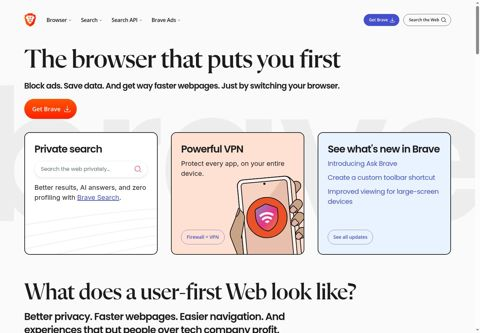
\includegraphics[width=\linewidth]{thumbnails/sql-run-1362-source.jpg}\par\footnotesize Original\end{minipage}\hfill
\begin{minipage}[t]{.47\linewidth}\vspace{0pt}\centering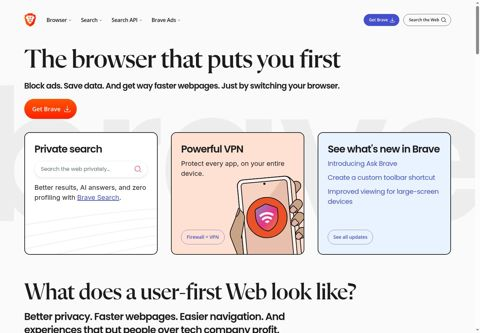
\includegraphics[width=\linewidth]{thumbnails/sql-run-1362-selected.jpg}\par\footnotesize Selected P5\end{minipage}\par\smallskip
{\footnotesize Route: P1/L > P2/L > P2/H > P1/H\par Planner: D; visual: Accepted.\par Usability checks: Accepted.}\end{minipage}\hfill\begin{minipage}[t]{.54\linewidth}\vspace{0pt}
\begingroup\footnotesize\setlength{\tabcolsep}{3pt}\renewcommand{\arraystretch}{1.14}
\noindent\begin{tabular*}{\linewidth}{@{\extracolsep{\fill}}p{0.4000\linewidth}p{\dimexpr0.3100\linewidth-2\tabcolsep\relax}p{\dimexpr0.2900\linewidth-2\tabcolsep\relax}@{}}\toprule
\raggedright\textbf{Measure} & \raggedright\textbf{P2 mean} & \raggedright\textbf{P5}\tabularnewline\midrule
\raggedright Axe / LH & \raggedright 0.0/98.7 & \raggedright 0/99\tabularnewline
\raggedright Syn/Sem/Lay & \raggedright 0.0/3.0/2.0 & \raggedright 0/3/2\tabularnewline
\raggedright Content \% & \raggedright 100.0 & \raggedright 100.0\tabularnewline
\raggedright USD & \raggedright 0.0391 & \raggedright 0.0994\tabularnewline
\raggedright Time (s) & \raggedright 367.8 & \raggedright 475.3\tabularnewline
\raggedright Tokens (K) & \raggedright 304.2 & \raggedright 821.2\tabularnewline
\bottomrule\end{tabular*}\endgroup\par\medskip

\end{minipage}\par
Text/link/image retention: 100/100/100\%; Syn/Sem/Lay coverage: 98.8/88.8/100.0\%; 9 recorded choices.\par
\end{minipage}\par\medskip
\clearpage
\section{Source evidence -- 4 to 6}

\noindent\begin{minipage}{\linewidth}
\subsection{consultant.ru -- run 1370}

{\small Source \#435; reference Axe 16 / Lighthouse 86.}\par\smallskip
\noindent\begin{minipage}[t]{.43\linewidth}\vspace{0pt}\centering
\begin{minipage}[t]{.47\linewidth}\vspace{0pt}\centering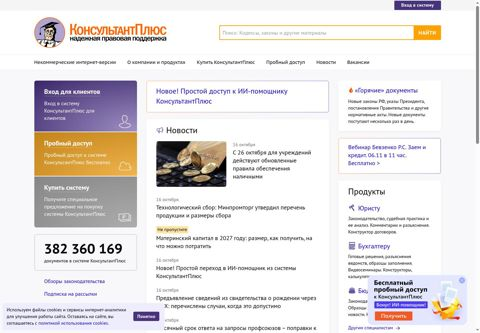
\includegraphics[width=\linewidth]{thumbnails/sql-run-1370-source.jpg}\par\footnotesize Original\end{minipage}\hfill
\begin{minipage}[t]{.47\linewidth}\vspace{0pt}\centering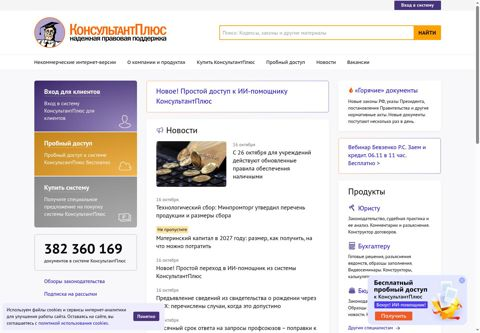
\includegraphics[width=\linewidth]{thumbnails/sql-run-1370-selected.jpg}\par\footnotesize Selected P5\end{minipage}\par\smallskip
{\footnotesize Route: P1/L\par Planner: D; visual: Accepted.\par Usability checks: Accepted.}\end{minipage}\hfill\begin{minipage}[t]{.54\linewidth}\vspace{0pt}
\begingroup\footnotesize\setlength{\tabcolsep}{3pt}\renewcommand{\arraystretch}{1.14}
\noindent\begin{tabular*}{\linewidth}{@{\extracolsep{\fill}}p{0.4000\linewidth}p{\dimexpr0.3100\linewidth-2\tabcolsep\relax}p{\dimexpr0.2900\linewidth-2\tabcolsep\relax}@{}}\toprule
\raggedright\textbf{Measure} & \raggedright\textbf{P2 mean} & \raggedright\textbf{P5}\tabularnewline\midrule
\raggedright Axe / LH & \raggedright 12.0/97.0 & \raggedright 12/97\tabularnewline
\raggedright Syn/Sem/Lay & \raggedright 12.0/0.0/4.0 & \raggedright 12/0/4\tabularnewline
\raggedright Content \% & \raggedright 100.0 & \raggedright 100.0\tabularnewline
\raggedright USD & \raggedright 0.0250 & \raggedright 0.1454\tabularnewline
\raggedright Time (s) & \raggedright 157.5 & \raggedright 418.7\tabularnewline
\raggedright Tokens (K) & \raggedright 189.9 & \raggedright 1,194.6\tabularnewline
\bottomrule\end{tabular*}\endgroup\par\medskip

\end{minipage}\par
Text/link/image retention: 100/100/100\%; Syn/Sem/Lay coverage: 100.0/93.8/99.6\%; 22 recorded choices.\par
\end{minipage}\par\medskip
\noindent\begin{minipage}{\linewidth}
\subsection{deviantart.com -- run 1369}

{\small Source \#480; reference Axe 4 / Lighthouse 96.}\par\smallskip
\noindent\begin{minipage}[t]{.43\linewidth}\vspace{0pt}\centering
\begin{minipage}[t]{.47\linewidth}\vspace{0pt}\centering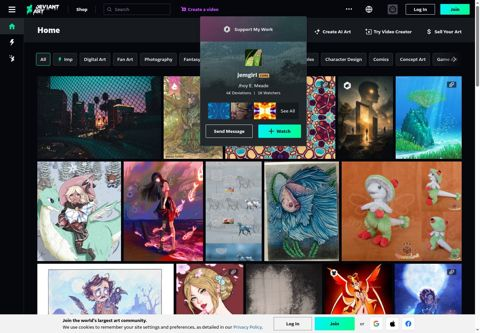
\includegraphics[width=\linewidth]{thumbnails/sql-run-1369-source.jpg}\par\footnotesize Original\end{minipage}\hfill
\begin{minipage}[t]{.47\linewidth}\vspace{0pt}\centering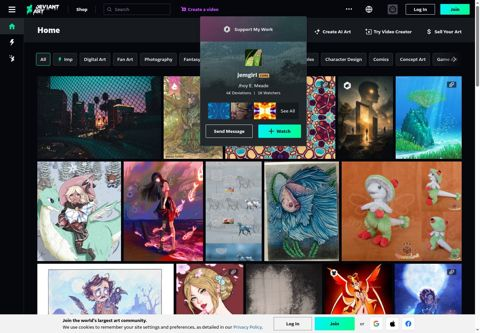
\includegraphics[width=\linewidth]{thumbnails/sql-run-1369-selected.jpg}\par\footnotesize Selected P5\end{minipage}\par\smallskip
{\footnotesize Route: P1/L\par Planner: D; visual: Accepted.\par Usability checks: Accepted.}\end{minipage}\hfill\begin{minipage}[t]{.54\linewidth}\vspace{0pt}
\begingroup\footnotesize\setlength{\tabcolsep}{3pt}\renewcommand{\arraystretch}{1.14}
\noindent\begin{tabular*}{\linewidth}{@{\extracolsep{\fill}}p{0.4000\linewidth}p{\dimexpr0.3100\linewidth-2\tabcolsep\relax}p{\dimexpr0.2900\linewidth-2\tabcolsep\relax}@{}}\toprule
\raggedright\textbf{Measure} & \raggedright\textbf{P2 mean} & \raggedright\textbf{P5}\tabularnewline\midrule
\raggedright Axe / LH & \raggedright 0.0/100.0 & \raggedright 0/100\tabularnewline
\raggedright Syn/Sem/Lay & \raggedright 0.0/11.0/1.0 & \raggedright 0/11/1\tabularnewline
\raggedright Content \% & \raggedright 100.0 & \raggedright 100.0\tabularnewline
\raggedright USD & \raggedright 0.0476 & \raggedright 0.0243\tabularnewline
\raggedright Time (s) & \raggedright 210.7 & \raggedright 89.4\tabularnewline
\raggedright Tokens (K) & \raggedright 401.9 & \raggedright 211.5\tabularnewline
\bottomrule\end{tabular*}\endgroup\par\medskip

\end{minipage}\par
Text/link/image retention: 100/100/100\%; Syn/Sem/Lay coverage: 99.6/74.8/96.4\%; 1 recorded choices.\par
\end{minipage}\par\medskip
\noindent\begin{minipage}{\linewidth}
\subsection{docker.com -- run 1365}

{\small Source \#364; reference Axe 18 / Lighthouse 88.}\par\smallskip
\noindent\begin{minipage}[t]{.43\linewidth}\vspace{0pt}\centering
\begin{minipage}[t]{.47\linewidth}\vspace{0pt}\centering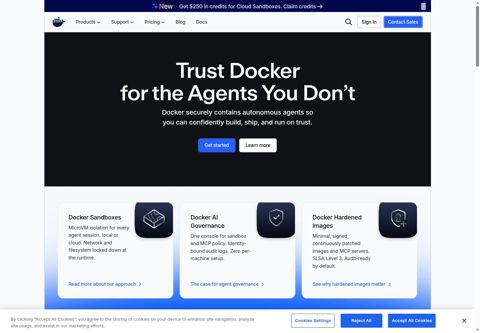
\includegraphics[width=\linewidth]{thumbnails/sql-run-1365-source.jpg}\par\footnotesize Original\end{minipage}\hfill
\begin{minipage}[t]{.47\linewidth}\vspace{0pt}\centering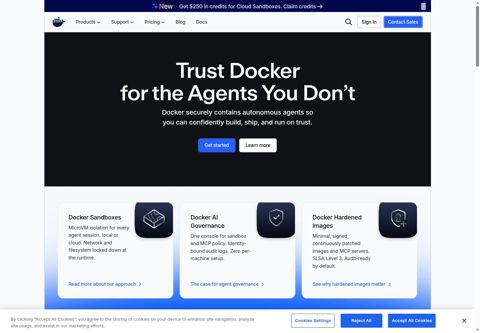
\includegraphics[width=\linewidth]{thumbnails/sql-run-1365-selected.jpg}\par\footnotesize Selected P5\end{minipage}\par\smallskip
{\footnotesize Route: P2/L > P2/H > P1/L\par Planner: D; visual: Accepted.\par Usability checks: Accepted.}\end{minipage}\hfill\begin{minipage}[t]{.54\linewidth}\vspace{0pt}
\begingroup\footnotesize\setlength{\tabcolsep}{3pt}\renewcommand{\arraystretch}{1.14}
\noindent\begin{tabular*}{\linewidth}{@{\extracolsep{\fill}}p{0.4000\linewidth}p{\dimexpr0.3100\linewidth-2\tabcolsep\relax}p{\dimexpr0.2900\linewidth-2\tabcolsep\relax}@{}}\toprule
\raggedright\textbf{Measure} & \raggedright\textbf{P2 mean} & \raggedright\textbf{P5}\tabularnewline\midrule
\raggedright Axe / LH & \raggedright 4.7/95.0 & \raggedright 1/98\tabularnewline
\raggedright Syn/Sem/Lay & \raggedright 3.7/11.3/2.0 & \raggedright 1/11/1\tabularnewline
\raggedright Content \% & \raggedright 100.0 & \raggedright 100.0\tabularnewline
\raggedright USD & \raggedright 0.1270 & \raggedright 0.2807\tabularnewline
\raggedright Time (s) & \raggedright 721.8 & \raggedright 842.7\tabularnewline
\raggedright Tokens (K) & \raggedright 1,044.3 & \raggedright 2,389.6\tabularnewline
\bottomrule\end{tabular*}\endgroup\par\medskip

\end{minipage}\par
Text/link/image retention: 100/100/100\%; Syn/Sem/Lay coverage: 100.0/82.5/93.9\%; 24 recorded choices.\par
\end{minipage}\par\medskip
\clearpage
\section{Source evidence -- 7 to 9}

\noindent\begin{minipage}{\linewidth}
\subsection{drom.ru -- run 1373}

{\small Source \#425; reference Axe 73 / Lighthouse 82.}\par\smallskip
\noindent\begin{minipage}[t]{.43\linewidth}\vspace{0pt}\centering
\begin{minipage}[t]{.47\linewidth}\vspace{0pt}\centering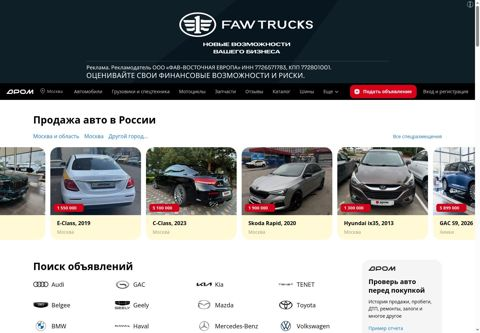
\includegraphics[width=\linewidth]{thumbnails/sql-run-1373-source.jpg}\par\footnotesize Original\end{minipage}\hfill
\begin{minipage}[t]{.47\linewidth}\vspace{0pt}\centering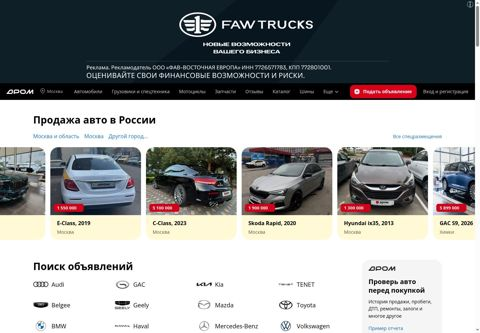
\includegraphics[width=\linewidth]{thumbnails/sql-run-1373-selected.jpg}\par\footnotesize Selected P5\end{minipage}\par\smallskip
{\footnotesize Route: P1/L > P2/L > P1/L > P2/L > P1/L\par Planner: D; visual: Accepted.\par Usability checks: Accepted.}\end{minipage}\hfill\begin{minipage}[t]{.54\linewidth}\vspace{0pt}
\begingroup\footnotesize\setlength{\tabcolsep}{3pt}\renewcommand{\arraystretch}{1.14}
\noindent\begin{tabular*}{\linewidth}{@{\extracolsep{\fill}}p{0.4000\linewidth}p{\dimexpr0.3100\linewidth-2\tabcolsep\relax}p{\dimexpr0.2900\linewidth-2\tabcolsep\relax}@{}}\toprule
\raggedright\textbf{Measure} & \raggedright\textbf{P2 mean} & \raggedright\textbf{P5}\tabularnewline\midrule
\raggedright Axe / LH & \raggedright 27.0/94.0 & \raggedright 3/98\tabularnewline
\raggedright Syn/Sem/Lay & \raggedright 3.0/4.0/32.0 & \raggedright 3/4/8\tabularnewline
\raggedright Content \% & \raggedright 100.0 & \raggedright 100.0\tabularnewline
\raggedright USD & \raggedright 0.0872 & \raggedright 0.1355\tabularnewline
\raggedright Time (s) & \raggedright 1,454.7 & \raggedright 711.0\tabularnewline
\raggedright Tokens (K) & \raggedright 709.9 & \raggedright 1,170.3\tabularnewline
\bottomrule\end{tabular*}\endgroup\par\medskip

\end{minipage}\par
Text/link/image retention: 100/100/100\%; Syn/Sem/Lay coverage: 99.4/94.7/93.4\%; 12 recorded choices.\par
\end{minipage}\par\medskip
\noindent\begin{minipage}{\linewidth}
\subsection{eventbrite.com -- run 1366}

{\small Source \#411; reference Axe 2 / Lighthouse 92.}\par\smallskip
\noindent\begin{minipage}[t]{.43\linewidth}\vspace{0pt}\centering
\begin{minipage}[t]{.47\linewidth}\vspace{0pt}\centering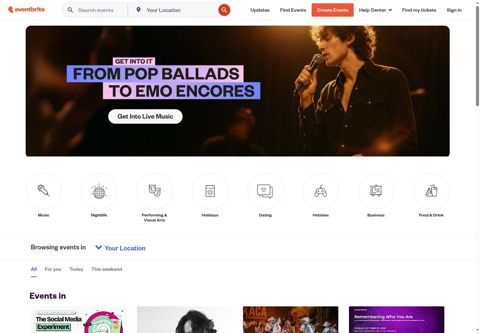
\includegraphics[width=\linewidth]{thumbnails/sql-run-1366-source.jpg}\par\footnotesize Original\end{minipage}\hfill
\begin{minipage}[t]{.47\linewidth}\vspace{0pt}\centering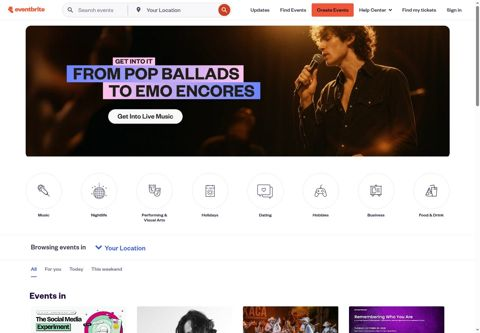
\includegraphics[width=\linewidth]{thumbnails/sql-run-1366-selected.jpg}\par\footnotesize Selected P5\end{minipage}\par\smallskip
{\footnotesize Route: P2/L\par Planner: D; visual: Accepted.\par Usability checks: Accepted.}\end{minipage}\hfill\begin{minipage}[t]{.54\linewidth}\vspace{0pt}
\begingroup\footnotesize\setlength{\tabcolsep}{3pt}\renewcommand{\arraystretch}{1.14}
\noindent\begin{tabular*}{\linewidth}{@{\extracolsep{\fill}}p{0.4000\linewidth}p{\dimexpr0.3100\linewidth-2\tabcolsep\relax}p{\dimexpr0.2900\linewidth-2\tabcolsep\relax}@{}}\toprule
\raggedright\textbf{Measure} & \raggedright\textbf{P2 mean} & \raggedright\textbf{P5}\tabularnewline\midrule
\raggedright Axe / LH & \raggedright 0.0/100.0 & \raggedright 0/100\tabularnewline
\raggedright Syn/Sem/Lay & \raggedright 0.0/45.7/30.0 & \raggedright 0/39/30\tabularnewline
\raggedright Content \% & \raggedright 100.0 & \raggedright 100.0\tabularnewline
\raggedright USD & \raggedright 0.0388 & \raggedright 0.0273\tabularnewline
\raggedright Time (s) & \raggedright 266.4 & \raggedright 76.8\tabularnewline
\raggedright Tokens (K) & \raggedright 323.9 & \raggedright 248.5\tabularnewline
\bottomrule\end{tabular*}\endgroup\par\medskip

\end{minipage}\par
Text/link/image retention: 100/100/100\%; Syn/Sem/Lay coverage: 97.0/82.9/99.8\%; 1 recorded choices.\par
\end{minipage}\par\medskip
\noindent\begin{minipage}{\linewidth}
\subsection{forbes.com -- run 1352}

{\small Source \#468; reference Axe 47 / Lighthouse 83.}\par\smallskip
\noindent\begin{minipage}[t]{.43\linewidth}\vspace{0pt}\centering
\begin{minipage}[t]{.47\linewidth}\vspace{0pt}\centering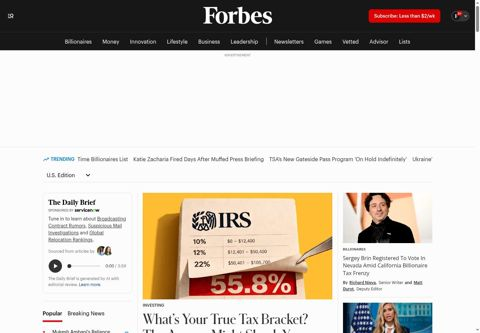
\includegraphics[width=\linewidth]{thumbnails/sql-run-1352-source.jpg}\par\footnotesize Original\end{minipage}\hfill
\begin{minipage}[t]{.47\linewidth}\vspace{0pt}\centering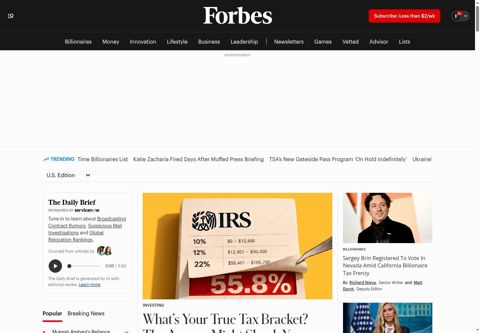
\includegraphics[width=\linewidth]{thumbnails/sql-run-1352-selected.jpg}\par\footnotesize Selected P5\end{minipage}\par\smallskip
{\footnotesize Route: P2/H\par Planner: D; visual: Accepted.\par Usability checks: Accepted.}\end{minipage}\hfill\begin{minipage}[t]{.54\linewidth}\vspace{0pt}
\begingroup\footnotesize\setlength{\tabcolsep}{3pt}\renewcommand{\arraystretch}{1.14}
\noindent\begin{tabular*}{\linewidth}{@{\extracolsep{\fill}}p{0.4000\linewidth}p{\dimexpr0.3100\linewidth-2\tabcolsep\relax}p{\dimexpr0.2900\linewidth-2\tabcolsep\relax}@{}}\toprule
\raggedright\textbf{Measure} & \raggedright\textbf{P2 mean} & \raggedright\textbf{P5}\tabularnewline\midrule
\raggedright Axe / LH & \raggedright 0.0/97.0 & \raggedright 0/99\tabularnewline
\raggedright Syn/Sem/Lay & \raggedright 0.0/44.0/1.3 & \raggedright 0/44/1\tabularnewline
\raggedright Content \% & \raggedright 100.0 & \raggedright 100.0\tabularnewline
\raggedright USD & \raggedright 0.7861 & \raggedright 0.7527\tabularnewline
\raggedright Time (s) & \raggedright 2,813.3 & \raggedright 2,025.8\tabularnewline
\raggedright Tokens (K) & \raggedright 7,425.1 & \raggedright 7,194.9\tabularnewline
\bottomrule\end{tabular*}\endgroup\par\medskip

\end{minipage}\par
Text/link/image retention: 100/100/100\%; Syn/Sem/Lay coverage: 99.8/91.5/98.2\%; 8 recorded choices.\par
\end{minipage}\par\medskip
\clearpage
\section{Source evidence -- 10 to 12}

\noindent\begin{minipage}{\linewidth}
\subsection{gandi.net -- run 1346}

{\small Source \#455; reference Axe 1 / Lighthouse 94.}\par\smallskip
\noindent\begin{minipage}[t]{.43\linewidth}\vspace{0pt}\centering
\begin{minipage}[t]{.47\linewidth}\vspace{0pt}\centering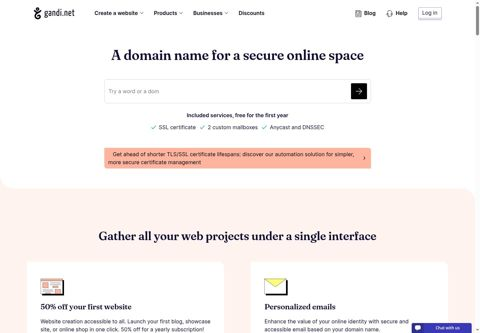
\includegraphics[width=\linewidth]{thumbnails/sql-run-1346-source.jpg}\par\footnotesize Original\end{minipage}\hfill
\begin{minipage}[t]{.47\linewidth}\vspace{0pt}\centering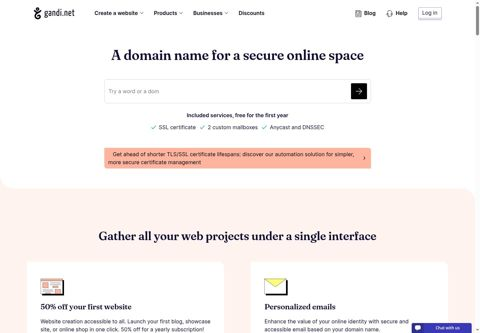
\includegraphics[width=\linewidth]{thumbnails/sql-run-1346-selected.jpg}\par\footnotesize Selected P5\end{minipage}\par\smallskip
{\footnotesize Route: P2/L > P2/H > P2/A\par Planner: D; visual: Accepted.\par Usability checks: Accepted.}\end{minipage}\hfill\begin{minipage}[t]{.54\linewidth}\vspace{0pt}
\begingroup\footnotesize\setlength{\tabcolsep}{3pt}\renewcommand{\arraystretch}{1.14}
\noindent\begin{tabular*}{\linewidth}{@{\extracolsep{\fill}}p{0.4000\linewidth}p{\dimexpr0.3100\linewidth-2\tabcolsep\relax}p{\dimexpr0.2900\linewidth-2\tabcolsep\relax}@{}}\toprule
\raggedright\textbf{Measure} & \raggedright\textbf{P2 mean} & \raggedright\textbf{P5}\tabularnewline\midrule
\raggedright Axe / LH & \raggedright 1.7/97.3 & \raggedright 0/99\tabularnewline
\raggedright Syn/Sem/Lay & \raggedright 1.7/10.7/0.0 & \raggedright 0/10/0\tabularnewline
\raggedright Content \% & \raggedright 100.0 & \raggedright 100.0\tabularnewline
\raggedright USD & \raggedright 0.0699 & \raggedright 0.2015\tabularnewline
\raggedright Time (s) & \raggedright 285.1 & \raggedright 936.6\tabularnewline
\raggedright Tokens (K) & \raggedright 578.4 & \raggedright 1,624.0\tabularnewline
\bottomrule\end{tabular*}\endgroup\par\medskip

\end{minipage}\par
Text/link/image retention: 100/100/100\%; Syn/Sem/Lay coverage: 98.7/80.7/100.0\%; 11 recorded choices.\par
\end{minipage}\par\medskip
\noindent\begin{minipage}{\linewidth}
\subsection{go.com -- run 1363}

{\small Source \#428; reference Axe 2 / Lighthouse 92.}\par\smallskip
\noindent\begin{minipage}[t]{.43\linewidth}\vspace{0pt}\centering
\begin{minipage}[t]{.47\linewidth}\vspace{0pt}\centering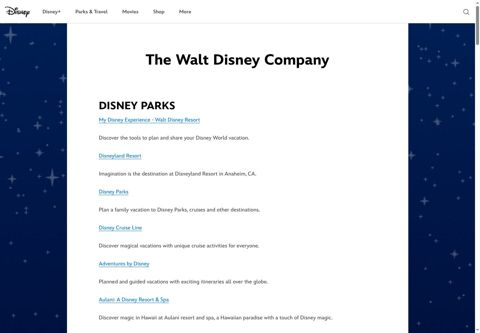
\includegraphics[width=\linewidth]{thumbnails/sql-run-1363-source.jpg}\par\footnotesize Original\end{minipage}\hfill
\begin{minipage}[t]{.47\linewidth}\vspace{0pt}\centering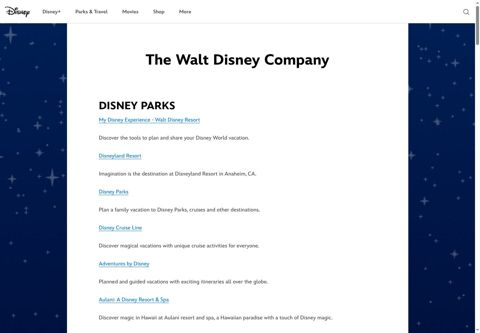
\includegraphics[width=\linewidth]{thumbnails/sql-run-1363-selected.jpg}\par\footnotesize Selected P5\end{minipage}\par\smallskip
{\footnotesize Route: P2/L\par Planner: D; visual: Accepted.\par Usability checks: Accepted.}\end{minipage}\hfill\begin{minipage}[t]{.54\linewidth}\vspace{0pt}
\begingroup\footnotesize\setlength{\tabcolsep}{3pt}\renewcommand{\arraystretch}{1.14}
\noindent\begin{tabular*}{\linewidth}{@{\extracolsep{\fill}}p{0.4000\linewidth}p{\dimexpr0.3100\linewidth-2\tabcolsep\relax}p{\dimexpr0.2900\linewidth-2\tabcolsep\relax}@{}}\toprule
\raggedright\textbf{Measure} & \raggedright\textbf{P2 mean} & \raggedright\textbf{P5}\tabularnewline\midrule
\raggedright Axe / LH & \raggedright 0.0/100.0 & \raggedright 0/100\tabularnewline
\raggedright Syn/Sem/Lay & \raggedright 0.0/7.0/0.0 & \raggedright 0/7/0\tabularnewline
\raggedright Content \% & \raggedright 100.0 & \raggedright 100.0\tabularnewline
\raggedright USD & \raggedright 0.0298 & \raggedright 0.0113\tabularnewline
\raggedright Time (s) & \raggedright 201.4 & \raggedright 61.6\tabularnewline
\raggedright Tokens (K) & \raggedright 238.6 & \raggedright 95.8\tabularnewline
\bottomrule\end{tabular*}\endgroup\par\medskip

\end{minipage}\par
Text/link/image retention: 100/100/100\%; Syn/Sem/Lay coverage: 100.0/82.2/100.0\%; 1 recorded choices.\par
\end{minipage}\par\medskip
\noindent\begin{minipage}{\linewidth}
\subsection{line.me -- run 1361}

{\small Source \#434; reference Axe 17 / Lighthouse 87.}\par\smallskip
\noindent\begin{minipage}[t]{.43\linewidth}\vspace{0pt}\centering
\begin{minipage}[t]{.47\linewidth}\vspace{0pt}\centering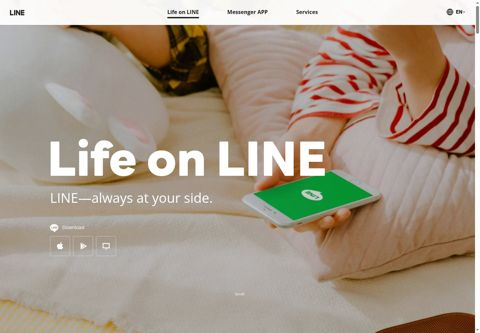
\includegraphics[width=\linewidth]{thumbnails/sql-run-1361-source.jpg}\par\footnotesize Original\end{minipage}\hfill
\begin{minipage}[t]{.47\linewidth}\vspace{0pt}\centering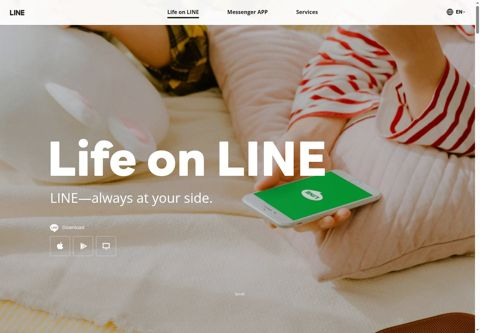
\includegraphics[width=\linewidth]{thumbnails/sql-run-1361-selected.jpg}\par\footnotesize Selected P5\end{minipage}\par\smallskip
{\footnotesize Route: P1/L > P2/L\par Planner: D; visual: Accepted.\par Usability checks: Accepted.}\end{minipage}\hfill\begin{minipage}[t]{.54\linewidth}\vspace{0pt}
\begingroup\footnotesize\setlength{\tabcolsep}{3pt}\renewcommand{\arraystretch}{1.14}
\noindent\begin{tabular*}{\linewidth}{@{\extracolsep{\fill}}p{0.4000\linewidth}p{\dimexpr0.3100\linewidth-2\tabcolsep\relax}p{\dimexpr0.2900\linewidth-2\tabcolsep\relax}@{}}\toprule
\raggedright\textbf{Measure} & \raggedright\textbf{P2 mean} & \raggedright\textbf{P5}\tabularnewline\midrule
\raggedright Axe / LH & \raggedright 6.0/95.3 & \raggedright 6/95\tabularnewline
\raggedright Syn/Sem/Lay & \raggedright 6.0/76.0/8.0 & \raggedright 6/76/8\tabularnewline
\raggedright Content \% & \raggedright 100.0 & \raggedright 100.0\tabularnewline
\raggedright USD & \raggedright 0.0574 & \raggedright 0.6832\tabularnewline
\raggedright Time (s) & \raggedright 696.9 & \raggedright 868.1\tabularnewline
\raggedright Tokens (K) & \raggedright 472.1 & \raggedright 6,403.9\tabularnewline
\bottomrule\end{tabular*}\endgroup\par\medskip

\end{minipage}\par
Text/link/image retention: 100/100/100\%; Syn/Sem/Lay coverage: 100.0/69.4/96.6\%; 30 recorded choices.\par
\end{minipage}\par\medskip
\clearpage
\section{Source evidence -- 13 to 15}

\noindent\begin{minipage}{\linewidth}
\subsection{linkedin.com -- run 1344}

{\small Source \#355; reference Axe 1 / Lighthouse 97.}\par\smallskip
\noindent\begin{minipage}[t]{.43\linewidth}\vspace{0pt}\centering
\begin{minipage}[t]{.47\linewidth}\vspace{0pt}\centering
\includegraphics[width=\linewidth]{thumbnails/sql-run-1344-source.jpg}\par\footnotesize Original\end{minipage}\hfill
\begin{minipage}[t]{.47\linewidth}\vspace{0pt}\centering
\includegraphics[width=\linewidth]{thumbnails/sql-run-1344-selected.jpg}\par\footnotesize Selected P5\end{minipage}\par\smallskip
{\footnotesize Route: P2/A\par Planner: D; visual: Accepted.\par Usability checks: Accepted.}\end{minipage}\hfill\begin{minipage}[t]{.54\linewidth}\vspace{0pt}
\begingroup\footnotesize\setlength{\tabcolsep}{3pt}\renewcommand{\arraystretch}{1.14}
\noindent\begin{tabular*}{\linewidth}{@{\extracolsep{\fill}}p{0.4000\linewidth}p{\dimexpr0.3100\linewidth-2\tabcolsep\relax}p{\dimexpr0.2900\linewidth-2\tabcolsep\relax}@{}}\toprule
\raggedright\textbf{Measure} & \raggedright\textbf{P2 mean} & \raggedright\textbf{P5}\tabularnewline\midrule
\raggedright Axe / LH & \raggedright 0.0/100.0 & \raggedright 0/100\tabularnewline
\raggedright Syn/Sem/Lay & \raggedright 0.0/3.3/0.0 & \raggedright 0/4/0\tabularnewline
\raggedright Content \% & \raggedright 100.0 & \raggedright 100.0\tabularnewline
\raggedright USD & \raggedright 0.0189 & \raggedright 0.0122\tabularnewline
\raggedright Time (s) & \raggedright 85.4 & \raggedright 55.2\tabularnewline
\raggedright Tokens (K) & \raggedright 147.4 & \raggedright 108.1\tabularnewline
\bottomrule\end{tabular*}\endgroup\par\medskip

\end{minipage}\par
Text/link/image retention: 100/100/100\%; Syn/Sem/Lay coverage: 100.0/80.9/77.0\%; 1 recorded choices.\par
\end{minipage}\par\medskip
\noindent\begin{minipage}{\linewidth}
\subsection{media.net -- run 1359}

{\small Source \#471; reference Axe 4 / Lighthouse 93.}\par\smallskip
\noindent\begin{minipage}[t]{.43\linewidth}\vspace{0pt}\centering
\begin{minipage}[t]{.47\linewidth}\vspace{0pt}\centering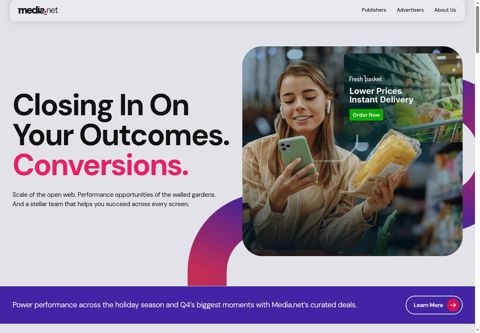
\includegraphics[width=\linewidth]{thumbnails/sql-run-1359-source.jpg}\par\footnotesize Original\end{minipage}\hfill
\begin{minipage}[t]{.47\linewidth}\vspace{0pt}\centering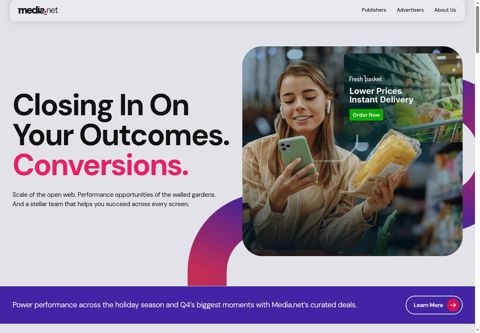
\includegraphics[width=\linewidth]{thumbnails/sql-run-1359-selected.jpg}\par\footnotesize Selected P5\end{minipage}\par\smallskip
{\footnotesize Route: P2/L\par Planner: D; visual: Accepted.\par Usability checks: Accepted.}\end{minipage}\hfill\begin{minipage}[t]{.54\linewidth}\vspace{0pt}
\begingroup\footnotesize\setlength{\tabcolsep}{3pt}\renewcommand{\arraystretch}{1.14}
\noindent\begin{tabular*}{\linewidth}{@{\extracolsep{\fill}}p{0.4000\linewidth}p{\dimexpr0.3100\linewidth-2\tabcolsep\relax}p{\dimexpr0.2900\linewidth-2\tabcolsep\relax}@{}}\toprule
\raggedright\textbf{Measure} & \raggedright\textbf{P2 mean} & \raggedright\textbf{P5}\tabularnewline\midrule
\raggedright Axe / LH & \raggedright 0.0/100.0 & \raggedright 0/100\tabularnewline
\raggedright Syn/Sem/Lay & \raggedright 0.0/6.0/1.0 & \raggedright 0/6/1\tabularnewline
\raggedright Content \% & \raggedright 100.0 & \raggedright 100.0\tabularnewline
\raggedright USD & \raggedright 0.0154 & \raggedright 0.0141\tabularnewline
\raggedright Time (s) & \raggedright 195.8 & \raggedright 99.4\tabularnewline
\raggedright Tokens (K) & \raggedright 123.3 & \raggedright 113.5\tabularnewline
\bottomrule\end{tabular*}\endgroup\par\medskip

\end{minipage}\par
Text/link/image retention: 100/100/100\%; Syn/Sem/Lay coverage: 100.0/92.2/100.0\%; 2 recorded choices.\par
\end{minipage}\par\medskip
\noindent\begin{minipage}{\linewidth}
\subsection{mikrotik.com -- run 1364}

{\small Source \#423; reference Axe 48 / Lighthouse 97.}\par\smallskip
\noindent\begin{minipage}[t]{.43\linewidth}\vspace{0pt}\centering
\begin{minipage}[t]{.47\linewidth}\vspace{0pt}\centering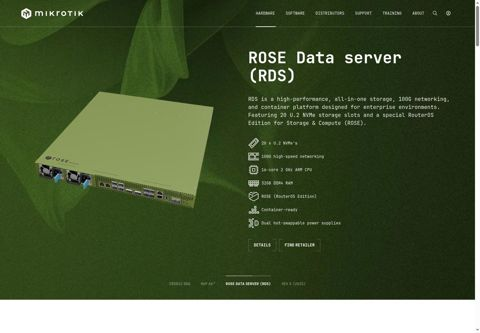
\includegraphics[width=\linewidth]{thumbnails/sql-run-1364-source.jpg}\par\footnotesize Original\end{minipage}\hfill
\begin{minipage}[t]{.47\linewidth}\vspace{0pt}\centering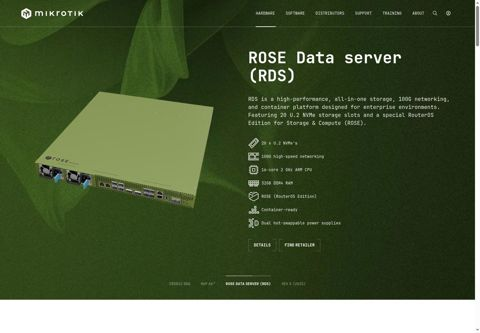
\includegraphics[width=\linewidth]{thumbnails/sql-run-1364-selected.jpg}\par\footnotesize Selected P5\end{minipage}\par\smallskip
{\footnotesize Route: P1/L\par Planner: D; visual: Accepted.\par Usability checks: Accepted.}\end{minipage}\hfill\begin{minipage}[t]{.54\linewidth}\vspace{0pt}
\begingroup\footnotesize\setlength{\tabcolsep}{3pt}\renewcommand{\arraystretch}{1.14}
\noindent\begin{tabular*}{\linewidth}{@{\extracolsep{\fill}}p{0.4000\linewidth}p{\dimexpr0.3100\linewidth-2\tabcolsep\relax}p{\dimexpr0.2900\linewidth-2\tabcolsep\relax}@{}}\toprule
\raggedright\textbf{Measure} & \raggedright\textbf{P2 mean} & \raggedright\textbf{P5}\tabularnewline\midrule
\raggedright Axe / LH & \raggedright 0.0/100.0 & \raggedright 0/100\tabularnewline
\raggedright Syn/Sem/Lay & \raggedright 0.0/28.7/7.0 & \raggedright 0/28/8\tabularnewline
\raggedright Content \% & \raggedright 100.0 & \raggedright 100.0\tabularnewline
\raggedright USD & \raggedright 0.0253 & \raggedright 0.0553\tabularnewline
\raggedright Time (s) & \raggedright 193.2 & \raggedright 207.8\tabularnewline
\raggedright Tokens (K) & \raggedright 209.9 & \raggedright 511.7\tabularnewline
\bottomrule\end{tabular*}\endgroup\par\medskip

\end{minipage}\par
Text/link/image retention: 100/100/100\%; Syn/Sem/Lay coverage: 100.0/86.2/87.7\%; 3 recorded choices.\par
\end{minipage}\par\medskip
\clearpage
\section{Source evidence -- 16 to 18}

\noindent\begin{minipage}{\linewidth}
\subsection{mts.ru -- run 1351}

{\small Source \#476; reference Axe 15 / Lighthouse 86.}\par\smallskip
\noindent\begin{minipage}[t]{.43\linewidth}\vspace{0pt}\centering
\begin{minipage}[t]{.47\linewidth}\vspace{0pt}\centering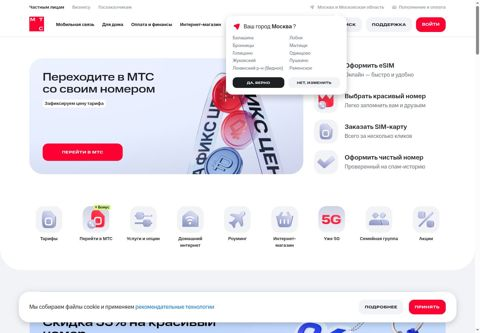
\includegraphics[width=\linewidth]{thumbnails/sql-run-1351-source.jpg}\par\footnotesize Original\end{minipage}\hfill
\begin{minipage}[t]{.47\linewidth}\vspace{0pt}\centering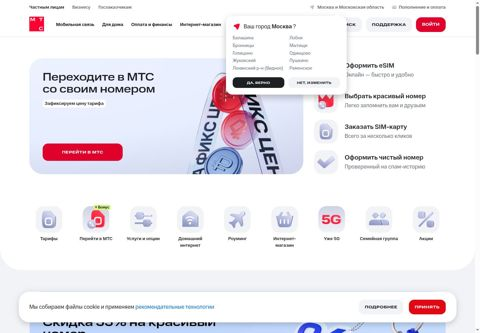
\includegraphics[width=\linewidth]{thumbnails/sql-run-1351-selected.jpg}\par\footnotesize Selected P5\end{minipage}\par\smallskip
{\footnotesize Route: P1/L\par Planner: D; visual: Accepted.\par Usability checks: Not accepted.}\end{minipage}\hfill\begin{minipage}[t]{.54\linewidth}\vspace{0pt}
\begingroup\footnotesize\setlength{\tabcolsep}{3pt}\renewcommand{\arraystretch}{1.14}
\noindent\begin{tabular*}{\linewidth}{@{\extracolsep{\fill}}p{0.4000\linewidth}p{\dimexpr0.3100\linewidth-2\tabcolsep\relax}p{\dimexpr0.2900\linewidth-2\tabcolsep\relax}@{}}\toprule
\raggedright\textbf{Measure} & \raggedright\textbf{P2 mean} & \raggedright\textbf{P5}\tabularnewline\midrule
\raggedright Axe / LH & \raggedright 0.3/98.7 & \raggedright 0/100\tabularnewline
\raggedright Syn/Sem/Lay & \raggedright 0.0/1.0/0.3 & \raggedright 0/1/0\tabularnewline
\raggedright Content \% & \raggedright 100.0 & \raggedright 100.0\tabularnewline
\raggedright USD & \raggedright 0.1231 & \raggedright 0.1041\tabularnewline
\raggedright Time (s) & \raggedright 817.0 & \raggedright 431.6\tabularnewline
\raggedright Tokens (K) & \raggedright 1,050.5 & \raggedright 908.4\tabularnewline
\bottomrule\end{tabular*}\endgroup\par\medskip

\end{minipage}\par
Text/link/image retention: 100/100/100\%; Syn/Sem/Lay coverage: 84.6/75.7/96.0\%; 5 recorded choices.\par
\end{minipage}\par\medskip
\noindent\begin{minipage}{\linewidth}
\subsection{mysql.com -- run 1367}

{\small Source \#390; reference Axe 51 / Lighthouse 83.}\par\smallskip
\noindent\begin{minipage}[t]{.43\linewidth}\vspace{0pt}\centering
\begin{minipage}[t]{.47\linewidth}\vspace{0pt}\centering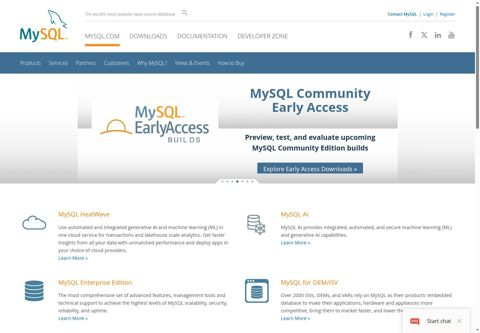
\includegraphics[width=\linewidth]{thumbnails/sql-run-1367-source.jpg}\par\footnotesize Original\end{minipage}\hfill
\begin{minipage}[t]{.47\linewidth}\vspace{0pt}\centering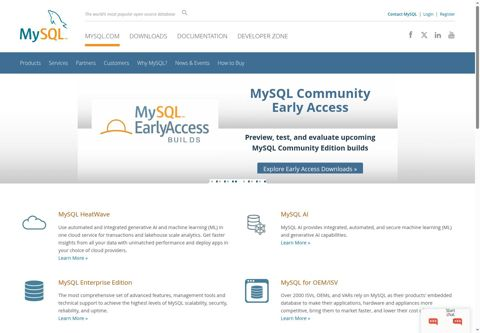
\includegraphics[width=\linewidth]{thumbnails/sql-run-1367-selected.jpg}\par\footnotesize Selected P5\end{minipage}\par\smallskip
{\footnotesize Route: P1/L > P2/H\par Planner: D; visual: Accepted.\par Usability checks: Not accepted.}\end{minipage}\hfill\begin{minipage}[t]{.54\linewidth}\vspace{0pt}
\begingroup\footnotesize\setlength{\tabcolsep}{3pt}\renewcommand{\arraystretch}{1.14}
\noindent\begin{tabular*}{\linewidth}{@{\extracolsep{\fill}}p{0.4000\linewidth}p{\dimexpr0.3100\linewidth-2\tabcolsep\relax}p{\dimexpr0.2900\linewidth-2\tabcolsep\relax}@{}}\toprule
\raggedright\textbf{Measure} & \raggedright\textbf{P2 mean} & \raggedright\textbf{P5}\tabularnewline\midrule
\raggedright Axe / LH & \raggedright 1.0/97.0 & \raggedright 1/97\tabularnewline
\raggedright Syn/Sem/Lay & \raggedright 0.0/7.7/3.0 & \raggedright 0/9/3\tabularnewline
\raggedright Content \% & \raggedright 100.0 & \raggedright 100.0\tabularnewline
\raggedright USD & \raggedright 0.1006 & \raggedright 0.2320\tabularnewline
\raggedright Time (s) & \raggedright 775.2 & \raggedright 1,406.5\tabularnewline
\raggedright Tokens (K) & \raggedright 825.4 & \raggedright 1,706.5\tabularnewline
\bottomrule\end{tabular*}\endgroup\par\medskip

\end{minipage}\par
Text/link/image retention: 100/100/100\%; Syn/Sem/Lay coverage: 99.5/96.3/98.2\%; 26 recorded choices.\par
\end{minipage}\par\medskip
\noindent\begin{minipage}{\linewidth}
\subsection{nginx.org -- run 1348}

{\small Source \#376; reference Axe 15 / Lighthouse 80.}\par\smallskip
\noindent\begin{minipage}[t]{.43\linewidth}\vspace{0pt}\centering
\begin{minipage}[t]{.47\linewidth}\vspace{0pt}\centering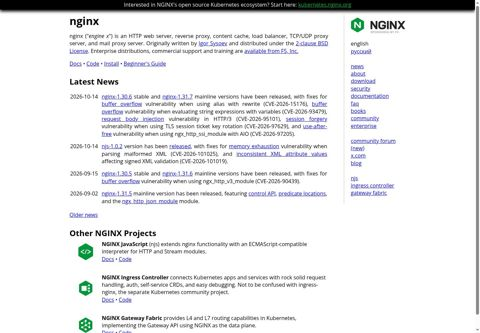
\includegraphics[width=\linewidth]{thumbnails/sql-run-1348-source.jpg}\par\footnotesize Original\end{minipage}\hfill
\begin{minipage}[t]{.47\linewidth}\vspace{0pt}\centering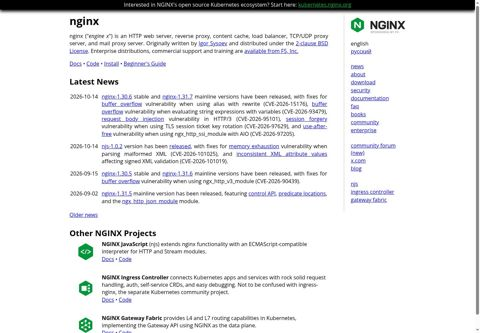
\includegraphics[width=\linewidth]{thumbnails/sql-run-1348-selected.jpg}\par\footnotesize Selected P5\end{minipage}\par\smallskip
{\footnotesize Route: P2/L\par Planner: D; visual: Accepted.\par Usability checks: Accepted.}\end{minipage}\hfill\begin{minipage}[t]{.54\linewidth}\vspace{0pt}
\begingroup\footnotesize\setlength{\tabcolsep}{3pt}\renewcommand{\arraystretch}{1.14}
\noindent\begin{tabular*}{\linewidth}{@{\extracolsep{\fill}}p{0.4000\linewidth}p{\dimexpr0.3100\linewidth-2\tabcolsep\relax}p{\dimexpr0.2900\linewidth-2\tabcolsep\relax}@{}}\toprule
\raggedright\textbf{Measure} & \raggedright\textbf{P2 mean} & \raggedright\textbf{P5}\tabularnewline\midrule
\raggedright Axe / LH & \raggedright 0.0/100.0 & \raggedright 0/100\tabularnewline
\raggedright Syn/Sem/Lay & \raggedright 0.0/0.3/0.0 & \raggedright 0/1/0\tabularnewline
\raggedright Content \% & \raggedright 100.0 & \raggedright 100.0\tabularnewline
\raggedright USD & \raggedright 0.0196 & \raggedright 0.0233\tabularnewline
\raggedright Time (s) & \raggedright 176.9 & \raggedright 159.1\tabularnewline
\raggedright Tokens (K) & \raggedright 130.1 & \raggedright 187.6\tabularnewline
\bottomrule\end{tabular*}\endgroup\par\medskip

\end{minipage}\par
Text/link/image retention: 100/100/100\%; Syn/Sem/Lay coverage: 100.0/89.2/100.0\%; 5 recorded choices.\par
\end{minipage}\par\medskip
\clearpage
\section{Source evidence -- 19 to 21}

\noindent\begin{minipage}{\linewidth}
\subsection{nist.gov -- run 1354}

{\small Source \#360; reference Axe 1 / Lighthouse 99.}\par\smallskip
\noindent\begin{minipage}[t]{.43\linewidth}\vspace{0pt}\centering
\begin{minipage}[t]{.47\linewidth}\vspace{0pt}\centering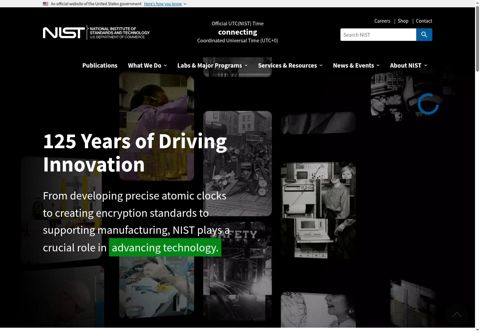
\includegraphics[width=\linewidth]{thumbnails/sql-run-1354-source.jpg}\par\footnotesize Original\end{minipage}\hfill
\begin{minipage}[t]{.47\linewidth}\vspace{0pt}\centering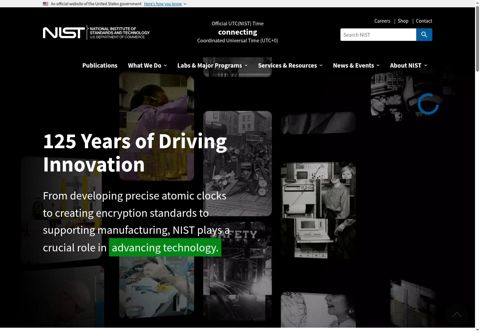
\includegraphics[width=\linewidth]{thumbnails/sql-run-1354-selected.jpg}\par\footnotesize Selected P5\end{minipage}\par\smallskip
{\footnotesize Route: P1/L > P2/L\par Planner: D; visual: Accepted.\par Usability checks: Accepted.}\end{minipage}\hfill\begin{minipage}[t]{.54\linewidth}\vspace{0pt}
\begingroup\footnotesize\setlength{\tabcolsep}{3pt}\renewcommand{\arraystretch}{1.14}
\noindent\begin{tabular*}{\linewidth}{@{\extracolsep{\fill}}p{0.4000\linewidth}p{\dimexpr0.3100\linewidth-2\tabcolsep\relax}p{\dimexpr0.2900\linewidth-2\tabcolsep\relax}@{}}\toprule
\raggedright\textbf{Measure} & \raggedright\textbf{P2 mean} & \raggedright\textbf{P5}\tabularnewline\midrule
\raggedright Axe / LH & \raggedright 0.0/100.0 & \raggedright 0/100\tabularnewline
\raggedright Syn/Sem/Lay & \raggedright 0.0/14.0/1.0 & \raggedright 0/14/1\tabularnewline
\raggedright Content \% & \raggedright 100.0 & \raggedright 100.0\tabularnewline
\raggedright USD & \raggedright 0.0172 & \raggedright 0.0212\tabularnewline
\raggedright Time (s) & \raggedright 138.0 & \raggedright 99.0\tabularnewline
\raggedright Tokens (K) & \raggedright 143.2 & \raggedright 186.1\tabularnewline
\bottomrule\end{tabular*}\endgroup\par\medskip

\end{minipage}\par
Text/link/image retention: 100/100/100\%; Syn/Sem/Lay coverage: 100.0/90.5/96.8\%; 2 recorded choices.\par
\end{minipage}\par\medskip
\noindent\begin{minipage}{\linewidth}
\subsection{php.net -- run 1358}

{\small Source \#377; reference Axe 2 / Lighthouse 95.}\par\smallskip
\noindent\begin{minipage}[t]{.43\linewidth}\vspace{0pt}\centering
\begin{minipage}[t]{.47\linewidth}\vspace{0pt}\centering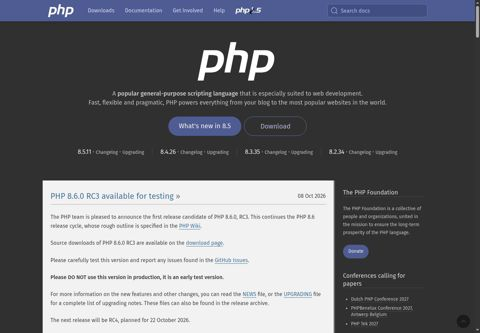
\includegraphics[width=\linewidth]{thumbnails/sql-run-1358-source.jpg}\par\footnotesize Original\end{minipage}\hfill
\begin{minipage}[t]{.47\linewidth}\vspace{0pt}\centering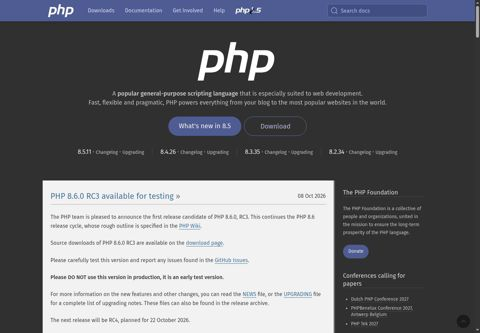
\includegraphics[width=\linewidth]{thumbnails/sql-run-1358-selected.jpg}\par\footnotesize Selected P5\end{minipage}\par\smallskip
{\footnotesize Route: P1/L\par Planner: D; visual: Accepted.\par Usability checks: Accepted.}\end{minipage}\hfill\begin{minipage}[t]{.54\linewidth}\vspace{0pt}
\begingroup\footnotesize\setlength{\tabcolsep}{3pt}\renewcommand{\arraystretch}{1.14}
\noindent\begin{tabular*}{\linewidth}{@{\extracolsep{\fill}}p{0.4000\linewidth}p{\dimexpr0.3100\linewidth-2\tabcolsep\relax}p{\dimexpr0.2900\linewidth-2\tabcolsep\relax}@{}}\toprule
\raggedright\textbf{Measure} & \raggedright\textbf{P2 mean} & \raggedright\textbf{P5}\tabularnewline\midrule
\raggedright Axe / LH & \raggedright 0.0/100.0 & \raggedright 0/100\tabularnewline
\raggedright Syn/Sem/Lay & \raggedright 0.0/3.0/4.0 & \raggedright 0/3/4\tabularnewline
\raggedright Content \% & \raggedright 100.0 & \raggedright 100.0\tabularnewline
\raggedright USD & \raggedright 0.0263 & \raggedright 0.0066\tabularnewline
\raggedright Time (s) & \raggedright 171.6 & \raggedright 50.6\tabularnewline
\raggedright Tokens (K) & \raggedright 221.9 & \raggedright 54.9\tabularnewline
\bottomrule\end{tabular*}\endgroup\par\medskip

\end{minipage}\par
Text/link/image retention: 100/100/100\%; Syn/Sem/Lay coverage: 100.0/85.6/100.0\%; 1 recorded choices.\par
\end{minipage}\par\medskip
\noindent\begin{minipage}{\linewidth}
\subsection{pubmatic.com -- run 1356}

{\small Source \#475; reference Axe 18 / Lighthouse 82.}\par\smallskip
\noindent\begin{minipage}[t]{.43\linewidth}\vspace{0pt}\centering
\begin{minipage}[t]{.47\linewidth}\vspace{0pt}\centering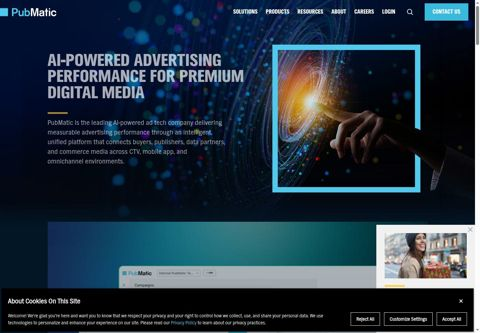
\includegraphics[width=\linewidth]{thumbnails/sql-run-1356-source.jpg}\par\footnotesize Original\end{minipage}\hfill
\begin{minipage}[t]{.47\linewidth}\vspace{0pt}\centering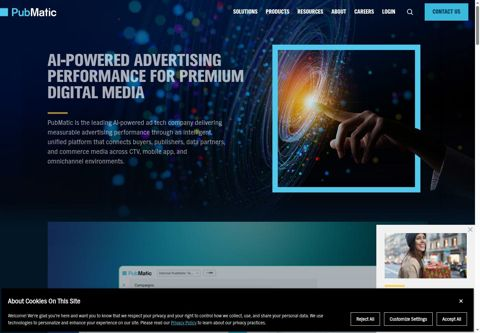
\includegraphics[width=\linewidth]{thumbnails/sql-run-1356-selected.jpg}\par\footnotesize Selected P5\end{minipage}\par\smallskip
{\footnotesize Route: P1/L > P2/L > P1/L\par Planner: D; visual: Accepted.\par Usability checks: Accepted.}\end{minipage}\hfill\begin{minipage}[t]{.54\linewidth}\vspace{0pt}
\begingroup\footnotesize\setlength{\tabcolsep}{3pt}\renewcommand{\arraystretch}{1.14}
\noindent\begin{tabular*}{\linewidth}{@{\extracolsep{\fill}}p{0.4000\linewidth}p{\dimexpr0.3100\linewidth-2\tabcolsep\relax}p{\dimexpr0.2900\linewidth-2\tabcolsep\relax}@{}}\toprule
\raggedright\textbf{Measure} & \raggedright\textbf{P2 mean} & \raggedright\textbf{P5}\tabularnewline\midrule
\raggedright Axe / LH & \raggedright 0.3/98.0 & \raggedright 0/99\tabularnewline
\raggedright Syn/Sem/Lay & \raggedright 0.0/5.0/8.3 & \raggedright 0/6/8\tabularnewline
\raggedright Content \% & \raggedright 100.0 & \raggedright 100.0\tabularnewline
\raggedright USD & \raggedright 0.0731 & \raggedright 0.1077\tabularnewline
\raggedright Time (s) & \raggedright 622.0 & \raggedright 424.9\tabularnewline
\raggedright Tokens (K) & \raggedright 569.8 & \raggedright 932.8\tabularnewline
\bottomrule\end{tabular*}\endgroup\par\medskip

\end{minipage}\par
Text/link/image retention: 100/100/100\%; Syn/Sem/Lay coverage: 100.0/84.7/91.3\%; 11 recorded choices.\par
\end{minipage}\par\medskip
\clearpage
\section{Source evidence -- 22 to 24}

\noindent\begin{minipage}{\linewidth}
\subsection{samsung.com -- run 1349}

{\small Source \#396; reference Axe 29 / Lighthouse 88.}\par\smallskip
\noindent\begin{minipage}[t]{.43\linewidth}\vspace{0pt}\centering
\begin{minipage}[t]{.47\linewidth}\vspace{0pt}\centering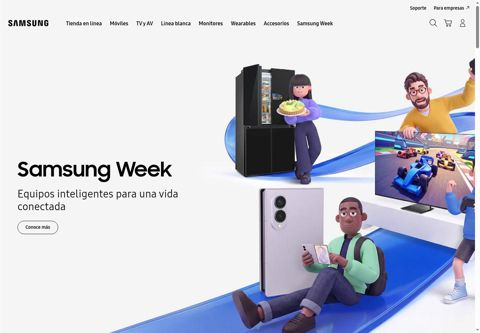
\includegraphics[width=\linewidth]{thumbnails/sql-run-1349-source.jpg}\par\footnotesize Original\end{minipage}\hfill
\begin{minipage}[t]{.47\linewidth}\vspace{0pt}\centering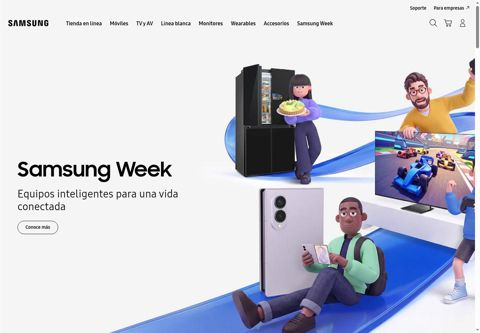
\includegraphics[width=\linewidth]{thumbnails/sql-run-1349-selected.jpg}\par\footnotesize Selected P5\end{minipage}\par\smallskip
{\footnotesize Route: P2/H\par Planner: D; visual: Accepted.\par Usability checks: Accepted.}\end{minipage}\hfill\begin{minipage}[t]{.54\linewidth}\vspace{0pt}
\begingroup\footnotesize\setlength{\tabcolsep}{3pt}\renewcommand{\arraystretch}{1.14}
\noindent\begin{tabular*}{\linewidth}{@{\extracolsep{\fill}}p{0.4000\linewidth}p{\dimexpr0.3100\linewidth-2\tabcolsep\relax}p{\dimexpr0.2900\linewidth-2\tabcolsep\relax}@{}}\toprule
\raggedright\textbf{Measure} & \raggedright\textbf{P2 mean} & \raggedright\textbf{P5}\tabularnewline\midrule
\raggedright Axe / LH & \raggedright 0.0/100.0 & \raggedright 0/100\tabularnewline
\raggedright Syn/Sem/Lay & \raggedright 0.0/29.7/2.0 & \raggedright 0/30/2\tabularnewline
\raggedright Content \% & \raggedright 100.0 & \raggedright 100.0\tabularnewline
\raggedright USD & \raggedright 0.3568 & \raggedright 0.0360\tabularnewline
\raggedright Time (s) & \raggedright 700.6 & \raggedright 144.8\tabularnewline
\raggedright Tokens (K) & \raggedright 1,630.4 & \raggedright 285.9\tabularnewline
\bottomrule\end{tabular*}\endgroup\par\medskip

\end{minipage}\par
Text/link/image retention: 100/100/100\%; Syn/Sem/Lay coverage: 99.9/68.7/99.4\%; 1 recorded choices.\par
\end{minipage}\par\medskip
\noindent\begin{minipage}{\linewidth}
\subsection{stripe.com -- run 1355}

{\small Source \#353; reference Axe 13 / Lighthouse 92.}\par\smallskip
\noindent\begin{minipage}[t]{.43\linewidth}\vspace{0pt}\centering
\begin{minipage}[t]{.47\linewidth}\vspace{0pt}\centering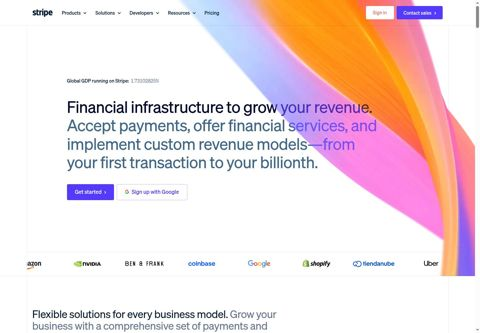
\includegraphics[width=\linewidth]{thumbnails/sql-run-1355-source.jpg}\par\footnotesize Original\end{minipage}\hfill
\begin{minipage}[t]{.47\linewidth}\vspace{0pt}\centering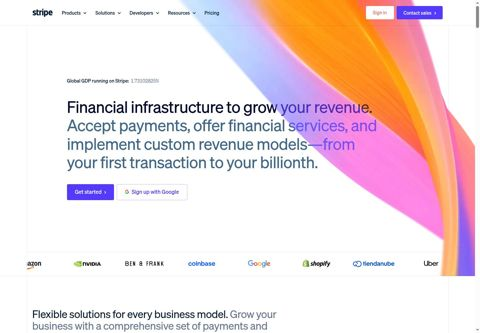
\includegraphics[width=\linewidth]{thumbnails/sql-run-1355-selected.jpg}\par\footnotesize Selected P5\end{minipage}\par\smallskip
{\footnotesize Route: P2/H\par Planner: D; visual: Accepted.\par Usability checks: Accepted.}\end{minipage}\hfill\begin{minipage}[t]{.54\linewidth}\vspace{0pt}
\begingroup\footnotesize\setlength{\tabcolsep}{3pt}\renewcommand{\arraystretch}{1.14}
\noindent\begin{tabular*}{\linewidth}{@{\extracolsep{\fill}}p{0.4000\linewidth}p{\dimexpr0.3100\linewidth-2\tabcolsep\relax}p{\dimexpr0.2900\linewidth-2\tabcolsep\relax}@{}}\toprule
\raggedright\textbf{Measure} & \raggedright\textbf{P2 mean} & \raggedright\textbf{P5}\tabularnewline\midrule
\raggedright Axe / LH & \raggedright 0.0/100.0 & \raggedright 0/100\tabularnewline
\raggedright Syn/Sem/Lay & \raggedright 0.0/18.3/9.0 & \raggedright 0/17/9\tabularnewline
\raggedright Content \% & \raggedright 100.0 & \raggedright 100.0\tabularnewline
\raggedright USD & \raggedright 0.1435 & \raggedright 0.0799\tabularnewline
\raggedright Time (s) & \raggedright 894.9 & \raggedright 492.1\tabularnewline
\raggedright Tokens (K) & \raggedright 1,223.0 & \raggedright 682.3\tabularnewline
\bottomrule\end{tabular*}\endgroup\par\medskip

\end{minipage}\par
Text/link/image retention: 100/100/100\%; Syn/Sem/Lay coverage: 100.0/72.1/91.7\%; 3 recorded choices.\par
\end{minipage}\par\medskip
\noindent\begin{minipage}{\linewidth}
\subsection{thenai.org -- run 1372}

{\small Source \#443; reference Axe 25 / Lighthouse 80.}\par\smallskip
\noindent\begin{minipage}[t]{.43\linewidth}\vspace{0pt}\centering
\begin{minipage}[t]{.47\linewidth}\vspace{0pt}\centering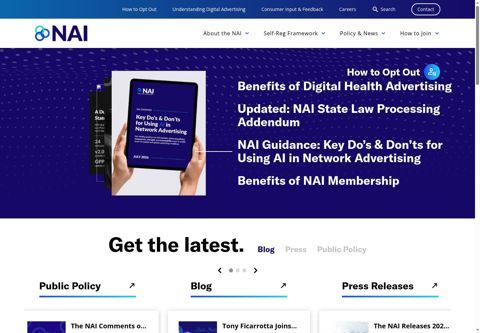
\includegraphics[width=\linewidth]{thumbnails/sql-run-1372-source.jpg}\par\footnotesize Original\end{minipage}\hfill
\begin{minipage}[t]{.47\linewidth}\vspace{0pt}\centering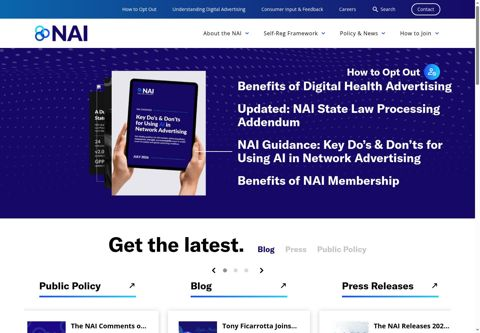
\includegraphics[width=\linewidth]{thumbnails/sql-run-1372-selected.jpg}\par\footnotesize Selected P5\end{minipage}\par\smallskip
{\footnotesize Route: P2/L\par Planner: D; visual: Accepted.\par Usability checks: Not accepted.}\end{minipage}\hfill\begin{minipage}[t]{.54\linewidth}\vspace{0pt}
\begingroup\footnotesize\setlength{\tabcolsep}{3pt}\renewcommand{\arraystretch}{1.14}
\noindent\begin{tabular*}{\linewidth}{@{\extracolsep{\fill}}p{0.4000\linewidth}p{\dimexpr0.3100\linewidth-2\tabcolsep\relax}p{\dimexpr0.2900\linewidth-2\tabcolsep\relax}@{}}\toprule
\raggedright\textbf{Measure} & \raggedright\textbf{P2 mean} & \raggedright\textbf{P5}\tabularnewline\midrule
\raggedright Axe / LH & \raggedright 2.7/97.0 & \raggedright 0/100\tabularnewline
\raggedright Syn/Sem/Lay & \raggedright 2.7/36.3/3.0 & \raggedright 0/35/3\tabularnewline
\raggedright Content \% & \raggedright 100.0 & \raggedright 100.0\tabularnewline
\raggedright USD & \raggedright 0.0996 & \raggedright 0.1163\tabularnewline
\raggedright Time (s) & \raggedright 565.1 & \raggedright 401.6\tabularnewline
\raggedright Tokens (K) & \raggedright 790.3 & \raggedright 1,010.4\tabularnewline
\bottomrule\end{tabular*}\endgroup\par\medskip

\end{minipage}\par
Text/link/image retention: 100/100/100\%; Syn/Sem/Lay coverage: 99.5/85.6/93.3\%; 5 recorded choices.\par
\end{minipage}\par\medskip
\clearpage
\section{Source evidence -- 25 to 27}

\noindent\begin{minipage}{\linewidth}
\subsection{time.com -- run 1368}

{\small Source \#358; reference Axe 10 / Lighthouse 91.}\par\smallskip
\noindent\begin{minipage}[t]{.43\linewidth}\vspace{0pt}\centering
\begin{minipage}[t]{.47\linewidth}\vspace{0pt}\centering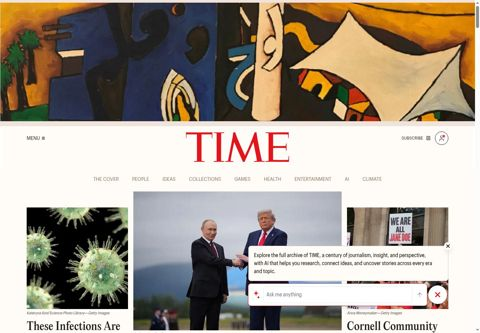
\includegraphics[width=\linewidth]{thumbnails/sql-run-1368-source.jpg}\par\footnotesize Original\end{minipage}\hfill
\begin{minipage}[t]{.47\linewidth}\vspace{0pt}\centering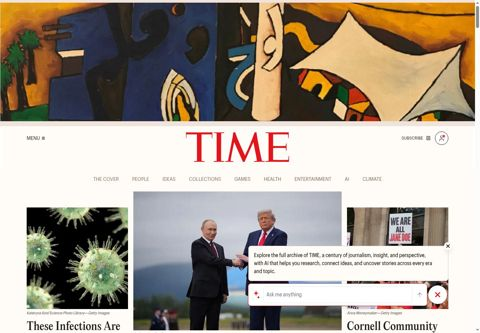
\includegraphics[width=\linewidth]{thumbnails/sql-run-1368-selected.jpg}\par\footnotesize Selected P5\end{minipage}\par\smallskip
{\footnotesize Route: P1/L > P2/L\par Planner: D; visual: Accepted.\par Usability checks: Accepted.}\end{minipage}\hfill\begin{minipage}[t]{.54\linewidth}\vspace{0pt}
\begingroup\footnotesize\setlength{\tabcolsep}{3pt}\renewcommand{\arraystretch}{1.14}
\noindent\begin{tabular*}{\linewidth}{@{\extracolsep{\fill}}p{0.4000\linewidth}p{\dimexpr0.3100\linewidth-2\tabcolsep\relax}p{\dimexpr0.2900\linewidth-2\tabcolsep\relax}@{}}\toprule
\raggedright\textbf{Measure} & \raggedright\textbf{P2 mean} & \raggedright\textbf{P5}\tabularnewline\midrule
\raggedright Axe / LH & \raggedright 0.0/99.7 & \raggedright 0/100\tabularnewline
\raggedright Syn/Sem/Lay & \raggedright 0.0/64.0/0.0 & \raggedright 0/64/0\tabularnewline
\raggedright Content \% & \raggedright 100.0 & \raggedright 100.0\tabularnewline
\raggedright USD & \raggedright 0.0750 & \raggedright 0.1096\tabularnewline
\raggedright Time (s) & \raggedright 540.0 & \raggedright 372.2\tabularnewline
\raggedright Tokens (K) & \raggedright 598.7 & \raggedright 1,005.2\tabularnewline
\bottomrule\end{tabular*}\endgroup\par\medskip

\end{minipage}\par
Text/link/image retention: 100/100/100\%; Syn/Sem/Lay coverage: 97.4/77.6/99.5\%; 3 recorded choices.\par
\end{minipage}\par\medskip
\noindent\begin{minipage}{\linewidth}
\subsection{tp-link.com -- run 1360}

{\small Source \#458; reference Axe 21 / Lighthouse 74; execution baseline 20/78.}\par\smallskip
\noindent\begin{minipage}[t]{.43\linewidth}\vspace{0pt}\centering
\begin{minipage}[t]{.47\linewidth}\vspace{0pt}\centering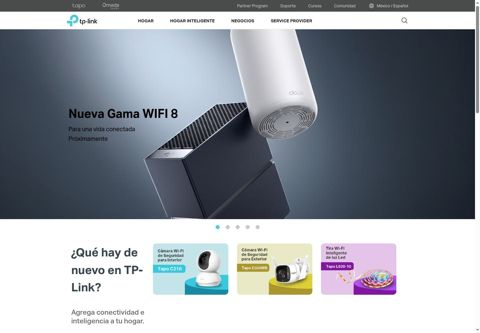
\includegraphics[width=\linewidth]{thumbnails/sql-run-1360-source.jpg}\par\footnotesize Original\end{minipage}\hfill
\begin{minipage}[t]{.47\linewidth}\vspace{0pt}\centering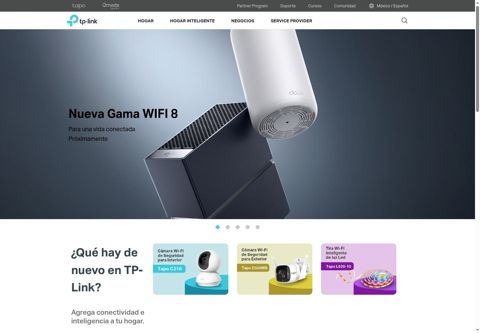
\includegraphics[width=\linewidth]{thumbnails/sql-run-1360-selected.jpg}\par\footnotesize Selected P5\end{minipage}\par\smallskip
{\footnotesize Route: P2/L > P1/H\par Planner: D; visual: Accepted.\par Usability checks: Accepted.}\end{minipage}\hfill\begin{minipage}[t]{.54\linewidth}\vspace{0pt}
\begingroup\footnotesize\setlength{\tabcolsep}{3pt}\renewcommand{\arraystretch}{1.14}
\noindent\begin{tabular*}{\linewidth}{@{\extracolsep{\fill}}p{0.4000\linewidth}p{\dimexpr0.3100\linewidth-2\tabcolsep\relax}p{\dimexpr0.2900\linewidth-2\tabcolsep\relax}@{}}\toprule
\raggedright\textbf{Measure} & \raggedright\textbf{P2 mean} & \raggedright\textbf{P5}\tabularnewline\midrule
\raggedright Axe / LH & \raggedright 2.7/91.3 & \raggedright 1/95\tabularnewline
\raggedright Syn/Sem/Lay & \raggedright 2.7/11.3/0.0 & \raggedright 1/10/0\tabularnewline
\raggedright Content \% & \raggedright 100.0 & \raggedright 100.0\tabularnewline
\raggedright USD & \raggedright 0.0536 & \raggedright 0.1172\tabularnewline
\raggedright Time (s) & \raggedright 292.2 & \raggedright 454.6\tabularnewline
\raggedright Tokens (K) & \raggedright 396.5 & \raggedright 966.1\tabularnewline
\bottomrule\end{tabular*}\endgroup\par\medskip

\end{minipage}\par
Text/link/image retention: 100/100/100\%; Syn/Sem/Lay coverage: 100.0/86.4/92.3\%; 12 recorded choices.\par
\end{minipage}\par\medskip
\noindent\begin{minipage}{\linewidth}
\subsection{triplinkintl.com -- run 1350}

{\small Source \#472; reference Axe 28 / Lighthouse 91.}\par\smallskip
\noindent\begin{minipage}[t]{.43\linewidth}\vspace{0pt}\centering
\begin{minipage}[t]{.47\linewidth}\vspace{0pt}\centering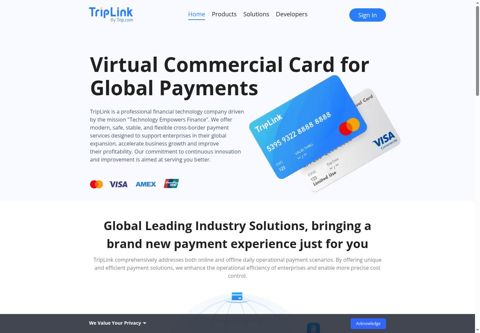
\includegraphics[width=\linewidth]{thumbnails/sql-run-1350-source.jpg}\par\footnotesize Original\end{minipage}\hfill
\begin{minipage}[t]{.47\linewidth}\vspace{0pt}\centering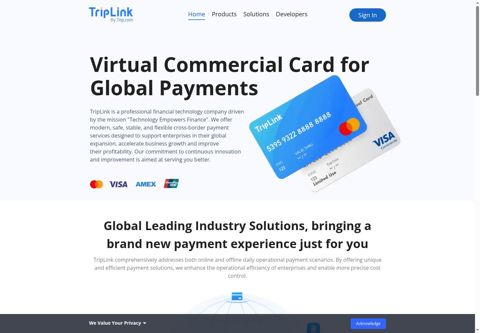
\includegraphics[width=\linewidth]{thumbnails/sql-run-1350-selected.jpg}\par\footnotesize Selected P5\end{minipage}\par\smallskip
{\footnotesize Route: P1/L\par Planner: D; visual: Accepted.\par Usability checks: Accepted.}\end{minipage}\hfill\begin{minipage}[t]{.54\linewidth}\vspace{0pt}
\begingroup\footnotesize\setlength{\tabcolsep}{3pt}\renewcommand{\arraystretch}{1.14}
\noindent\begin{tabular*}{\linewidth}{@{\extracolsep{\fill}}p{0.4000\linewidth}p{\dimexpr0.3100\linewidth-2\tabcolsep\relax}p{\dimexpr0.2900\linewidth-2\tabcolsep\relax}@{}}\toprule
\raggedright\textbf{Measure} & \raggedright\textbf{P2 mean} & \raggedright\textbf{P5}\tabularnewline\midrule
\raggedright Axe / LH & \raggedright 0.0/100.0 & \raggedright 0/100\tabularnewline
\raggedright Syn/Sem/Lay & \raggedright 0.0/1.0/5.0 & \raggedright 0/1/5\tabularnewline
\raggedright Content \% & \raggedright 100.0 & \raggedright 100.0\tabularnewline
\raggedright USD & \raggedright 0.0326 & \raggedright 0.0689\tabularnewline
\raggedright Time (s) & \raggedright 255.3 & \raggedright 377.5\tabularnewline
\raggedright Tokens (K) & \raggedright 265.7 & \raggedright 602.7\tabularnewline
\bottomrule\end{tabular*}\endgroup\par\medskip

\end{minipage}\par
Text/link/image retention: 100/100/100\%; Syn/Sem/Lay coverage: 100.0/87.9/98.9\%; 9 recorded choices.\par
\end{minipage}\par\medskip
\clearpage
\section{Source evidence -- 28 to 30}

\noindent\begin{minipage}{\linewidth}
\subsection{ubuntu.com -- run 1353}

{\small Source \#456; reference Axe 15 / Lighthouse 88.}\par\smallskip
\noindent\begin{minipage}[t]{.43\linewidth}\vspace{0pt}\centering
\begin{minipage}[t]{.47\linewidth}\vspace{0pt}\centering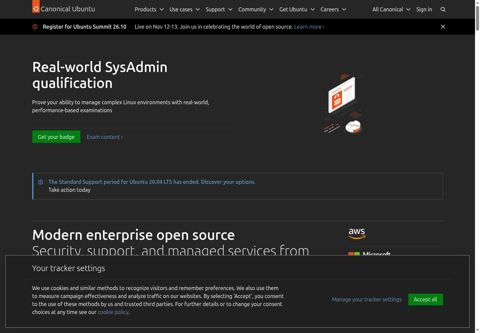
\includegraphics[width=\linewidth]{thumbnails/sql-run-1353-source.jpg}\par\footnotesize Original\end{minipage}\hfill
\begin{minipage}[t]{.47\linewidth}\vspace{0pt}\centering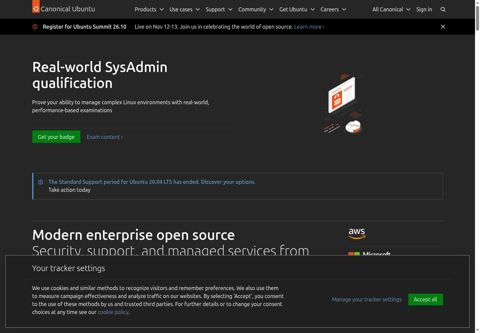
\includegraphics[width=\linewidth]{thumbnails/sql-run-1353-selected.jpg}\par\footnotesize Selected P5\end{minipage}\par\smallskip
{\footnotesize Route: P2/L\par Planner: D; visual: Accepted.\par Usability checks: Accepted.}\end{minipage}\hfill\begin{minipage}[t]{.54\linewidth}\vspace{0pt}
\begingroup\footnotesize\setlength{\tabcolsep}{3pt}\renewcommand{\arraystretch}{1.14}
\noindent\begin{tabular*}{\linewidth}{@{\extracolsep{\fill}}p{0.4000\linewidth}p{\dimexpr0.3100\linewidth-2\tabcolsep\relax}p{\dimexpr0.2900\linewidth-2\tabcolsep\relax}@{}}\toprule
\raggedright\textbf{Measure} & \raggedright\textbf{P2 mean} & \raggedright\textbf{P5}\tabularnewline\midrule
\raggedright Axe / LH & \raggedright 0.0/100.0 & \raggedright 0/100\tabularnewline
\raggedright Syn/Sem/Lay & \raggedright 0.0/9.3/0.0 & \raggedright 0/10/0\tabularnewline
\raggedright Content \% & \raggedright 100.0 & \raggedright 100.0\tabularnewline
\raggedright USD & \raggedright 0.1548 & \raggedright 0.0422\tabularnewline
\raggedright Time (s) & \raggedright 668.7 & \raggedright 238.9\tabularnewline
\raggedright Tokens (K) & \raggedright 758.3 & \raggedright 347.9\tabularnewline
\bottomrule\end{tabular*}\endgroup\par\medskip

\end{minipage}\par
Text/link/image retention: 100/100/100\%; Syn/Sem/Lay coverage: 100.0/45.8/99.8\%; 1 recorded choices.\par
\end{minipage}\par\medskip
\noindent\begin{minipage}{\linewidth}
\subsection{whatsapp.com -- run 1347}

{\small Source \#463; reference Axe 2 / Lighthouse 98.}\par\smallskip
\noindent\begin{minipage}[t]{.43\linewidth}\vspace{0pt}\centering
\begin{minipage}[t]{.47\linewidth}\vspace{0pt}\centering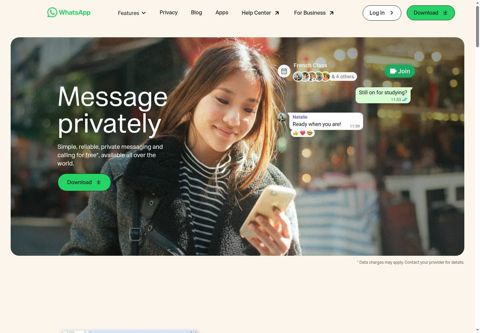
\includegraphics[width=\linewidth]{thumbnails/sql-run-1347-source.jpg}\par\footnotesize Original\end{minipage}\hfill
\begin{minipage}[t]{.47\linewidth}\vspace{0pt}\centering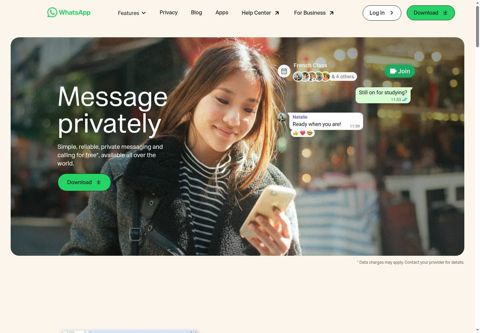
\includegraphics[width=\linewidth]{thumbnails/sql-run-1347-selected.jpg}\par\footnotesize Selected P5\end{minipage}\par\smallskip
{\footnotesize Route: P2/H\par Planner: D; visual: Accepted.\par Usability checks: Accepted.}\end{minipage}\hfill\begin{minipage}[t]{.54\linewidth}\vspace{0pt}
\begingroup\footnotesize\setlength{\tabcolsep}{3pt}\renewcommand{\arraystretch}{1.14}
\noindent\begin{tabular*}{\linewidth}{@{\extracolsep{\fill}}p{0.4000\linewidth}p{\dimexpr0.3100\linewidth-2\tabcolsep\relax}p{\dimexpr0.2900\linewidth-2\tabcolsep\relax}@{}}\toprule
\raggedright\textbf{Measure} & \raggedright\textbf{P2 mean} & \raggedright\textbf{P5}\tabularnewline\midrule
\raggedright Axe / LH & \raggedright 0.0/100.0 & \raggedright 0/100\tabularnewline
\raggedright Syn/Sem/Lay & \raggedright 0.0/57.0/2.0 & \raggedright 0/57/2\tabularnewline
\raggedright Content \% & \raggedright 100.0 & \raggedright 100.0\tabularnewline
\raggedright USD & \raggedright 0.1150 & \raggedright 0.0257\tabularnewline
\raggedright Time (s) & \raggedright 402.6 & \raggedright 153.6\tabularnewline
\raggedright Tokens (K) & \raggedright 911.9 & \raggedright 195.3\tabularnewline
\bottomrule\end{tabular*}\endgroup\par\medskip

\end{minipage}\par
Text/link/image retention: 100/100/100\%; Syn/Sem/Lay coverage: 99.8/93.2/100.0\%; 1 recorded choices.\par
\end{minipage}\par\medskip
\noindent\begin{minipage}{\linewidth}
\subsection{wps.com -- run 1371}

{\small Source \#452; reference Axe 18 / Lighthouse 86.}\par\smallskip
\noindent\begin{minipage}[t]{.43\linewidth}\vspace{0pt}\centering
\begin{minipage}[t]{.47\linewidth}\vspace{0pt}\centering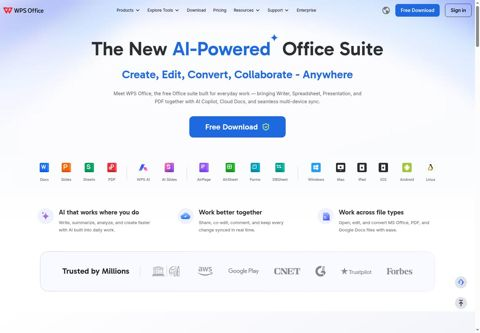
\includegraphics[width=\linewidth]{thumbnails/sql-run-1371-source.jpg}\par\footnotesize Original\end{minipage}\hfill
\begin{minipage}[t]{.47\linewidth}\vspace{0pt}\centering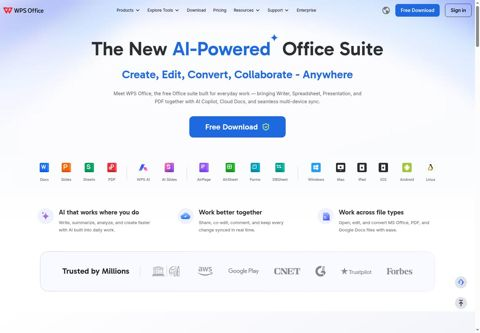
\includegraphics[width=\linewidth]{thumbnails/sql-run-1371-selected.jpg}\par\footnotesize Selected P5\end{minipage}\par\smallskip
{\footnotesize Route: P1/L > P1/H > P1/A\par Planner: D; visual: Accepted.\par Usability checks: Accepted.}\end{minipage}\hfill\begin{minipage}[t]{.54\linewidth}\vspace{0pt}
\begingroup\footnotesize\setlength{\tabcolsep}{3pt}\renewcommand{\arraystretch}{1.14}
\noindent\begin{tabular*}{\linewidth}{@{\extracolsep{\fill}}p{0.4000\linewidth}p{\dimexpr0.3100\linewidth-2\tabcolsep\relax}p{\dimexpr0.2900\linewidth-2\tabcolsep\relax}@{}}\toprule
\raggedright\textbf{Measure} & \raggedright\textbf{P2 mean} & \raggedright\textbf{P5}\tabularnewline\midrule
\raggedright Axe / LH & \raggedright 2.0/96.7 & \raggedright 7/94\tabularnewline
\raggedright Syn/Sem/Lay & \raggedright 0.0/13.0/14.0 & \raggedright 0/13/19\tabularnewline
\raggedright Content \% & \raggedright 100.0 & \raggedright 100.0\tabularnewline
\raggedright USD & \raggedright 0.1674 & \raggedright 0.1893\tabularnewline
\raggedright Time (s) & \raggedright 1,272.0 & \raggedright 525.5\tabularnewline
\raggedright Tokens (K) & \raggedright 1,523.5 & \raggedright 1,771.5\tabularnewline
\bottomrule\end{tabular*}\endgroup\par\medskip

\end{minipage}\par
Text/link/image retention: 100/100/100\%; Syn/Sem/Lay coverage: 100.0/54.3/98.3\%; 8 recorded choices.\par
\end{minipage}\par\medskip
\clearpage
\section{Resources, accounting, and traceability}

\begingroup\footnotesize\setlength{\tabcolsep}{3pt}\renewcommand{\arraystretch}{1.14}
\noindent\begin{tabular*}{\linewidth}{@{\extracolsep{\fill}}p{0.3000\linewidth}p{\dimexpr0.1000\linewidth-2\tabcolsep\relax}p{\dimexpr0.2200\linewidth-2\tabcolsep\relax}p{\dimexpr0.2200\linewidth-2\tabcolsep\relax}p{\dimexpr0.1600\linewidth-2\tabcolsep\relax}@{}}\toprule
\raggedright\textbf{Recorded task} & \raggedright\textbf{Calls} & \raggedright\textbf{Input tokens} & \raggedright\textbf{Output tokens} & \raggedright\textbf{USD}\tabularnewline\midrule
\raggedright Component planning & \raggedright 50 & \raggedright 388,889 & \raggedright 45,468 & \raggedright 0.069198\tabularnewline
\raggedright Contextual assessment & \raggedright 528 & \raggedright 10,049,793 & \raggedright 0 & \raggedright 1.004979\tabularnewline
\raggedright Diagnosis & \raggedright 130 & \raggedright 1,897,136 & \raggedright 131,314 & \raggedright 0.295365\tabularnewline
\raggedright Image alternatives & \raggedright 25 & \raggedright 233,844 & \raggedright 3,676 & \raggedright 0.031067\tabularnewline
\raggedright Repair generation & \raggedright 232 & \raggedright 7,158,300 & \raggedright 277,568 & \raggedright 1.002887\tabularnewline
\raggedright Route planning & \raggedright 241 & \raggedright 11,986,162 & \raggedright 0 & \raggedright 1.198616\tabularnewline
\raggedright Visual verification & \raggedright 128 & \raggedright 3,942,991 & \raggedright 20,462 & \raggedright 0.503095\tabularnewline
\bottomrule\end{tabular*}\endgroup\par\medskip

Execution costs cover every planning, generation and assessment request in the thirty selected executions, totaling US\$4.105208. accounting.csv links each run's cost to its recorded call charges and operational duration. Time is measured in seconds for the complete workflow; provider-request durations are recorded separately.

\subsection{Evidence map}

runs.csv and sources.csv bind the selected outputs and captures to exact frozen inputs. iterations.csv preserves evaluated versions for traceability. decisions.json records the closed choices, while prompts.csv links completed planning and repair requests. task-accounting.csv preserves complete task resources. The 450 source-matched fixed endpoints remain in fixed-conditions.csv.

The source panels report the selected outputs. Visual rationales, source hashes, model settings and request/response identities link these results to their supporting evidence. Rebuilding this report reads those files without running models, acquiring pages, or altering reviews.

\end{document}
